% 文档类
\documentclass[13pt]{ctexart}
% 设置页面
\usepackage{geometry}
\geometry{left = 3.5cm,right = 3.5cm,top=0cm}
% 设置标题 重命名为英文
\renewcommand{\figurename}{Figure}
\renewcommand{\tablename}{Table}
% 设置图表标题剧中对齐
\usepackage[justification=centering, singlelinecheck=false]{caption}
% 设置摘要页缩减
\usepackage{changepage}
% 设置目录换名
\renewcommand{\contentsname}{Contents}
% 设置摘要页表格
\usepackage{array}
\newcolumntype{L}[1]{>{\raggedright\let\newline\\\arraybackslash\hspace{0pt}}m{#1}}
\newcolumntype{C}[1]{>{\centering\let\newline\\\arraybackslash\hspace{0pt}}m{#1}}
\newcolumntype{R}[1]{>{\raggedleft\let\newline\\\arraybackslash\hspace{0pt}}m{#1}}
% 设置页眉页脚
\usepackage{fancyhdr}
% xelatex 调用系统字体 后者高亮插入代码
\usepackage{fontspec, listings}
% 设置等宽的代码字体
\setmonofont{Courier New}
% 清空页眉页脚
\pagestyle{fancy}
% 画箭头
\usepackage{stmaryrd}
% 插图片
\usepackage{graphicx}
% 数学符号中的绝对值
\usepackage{mathtools}
\DeclarePairedDelimiter\abs{\lvert}{\rvert}%
% 设置列表缩进
\usepackage[shortlabels]{enumitem}
% 排版长表格
\usepackage{tabularx}
% 合并表格的行
\usepackage{multirow}
% 引入网站作为参考文献
\usepackage{url}
% 随机生成一段话
\usepackage{lipsum}
% 修改目录标题距离
\usepackage[titles]{tocloft}
% 返回最后一页的页码
\usepackage{lastpage}
% 使用数学宏包
\usepackage{amsmath}
% 下划线宏包
\usepackage{ulem}
% 三线表宏包
\usepackage{booktabs}
% 调节表格行列间距 floatrowsep 写的不是很好
\usepackage{floatrow}
% 浮动盒子 摆脱浮动体设置,但排版不便,论文内可不设置
\usepackage{float}
% 修改表格标题位置 可能某个宏包冲突,得修正一下,理论上不必
\floatstyle{plaintop}
\restylefloat{table}
% 颜色
\usepackage{xcolor}
% 设置产考文献不输出默认名
\usepackage{etoolbox}
\patchcmd{\thebibliography}{\section*{\refname}}{}{}{}
% 设置字体
\usepackage{fontspec}
%\newcommand{\tnr}{\fontspec{Times New Roman}}
%\newcommand{\Georgia}{\fontspec{Georgia}}
%%fontspec下这个命令设置全局默认字体
%\setmainfont{TeX Gyre Pagella}
% 数学花体
\usepackage{amssymb}
% 设置两端对齐的宏包
\usepackage{ragged2e}
% 设置首行缩进
\usepackage{indentfirst}
% 伪粗体,不推荐使用
\usepackage{bm}
% 设置修改默认的section标题大小
\usepackage{titlesec}
\titleformat*{\section}{\LARGE\bfseries}
\titleformat*{\subsection}{\Large\bfseries}
\titleformat*{\subsubsection}{\Large\bfseries}
% 设置标题与上下文间距
\titlespacing*{\section}{0pt}{5.5ex plus 1ex minus .2ex}{4.3ex plus .2ex}
\titlespacing*{\subsection}{0pt}{2.5ex plus 1ex minus .2ex}{2.3ex plus .2ex}
\titlespacing*{\section}{0pt}{0.8ex}{0.8ex}
\titlespacing*{\subsection}{0pt}{0.6ex}{0.6ex}
\titlespacing*{\subsubsection}{0pt}{0.6ex}{0.6ex}
% 代码高亮方案宏包
\usepackage{listings}
\definecolor{CPPLight}  {HTML} {686868}
\definecolor{CPPSteel}  {HTML} {888888}
\definecolor{CPPDark}   {HTML} {262626}
\definecolor{CPPBlue}   {HTML} {4172A3}
\definecolor{CPPGreen}  {HTML} {487818}
\definecolor{CPPBrown}  {HTML} {A07040}
\definecolor{CPPRed}    {HTML} {AD4D3A}
\definecolor{CPPViolet} {HTML} {7040A0}
\definecolor{CPPGray}  {HTML} {B8B8B8}
\lstset{
	basicstyle=\ttfamily,
	breaklines=true,
	framextopmargin=50pt,
	frame=bottomline,
	columns=fixed,
	%numbers=left,                                       % 在左侧显示行号
	frame=none,                                          % 不显示背景边框
	backgroundcolor=\color[RGB]{255,255,255},            % 设定背景颜色
	keywordstyle=\color[RGB]{40,40,255},                 % 设定关键字颜色
	numberstyle=\footnotesize\color{darkgray},           % 设定行号格式
	commentstyle=\itshape\color[RGB]{0,96,96},                % 设置代码注释的格式
	stringstyle=\slshape\color[RGB]{128,0,0},   % 设置字符串格式
	showstringspaces=false,                              % 不显示字符串中的空格
	language=python,                                     % 设置语言
	morekeywords={alignas,continute,friend,register,true,alignof,decltype,goto,
		reinterpret_cast,try,asm,defult,if,return,typedef,auto,delete,inline,short,
		typeid,bool,do,int,signed,typename,break,double,long,sizeof,union,case,
		dynamic_cast,mutable,static,unsigned,catch,else,namespace,static_assert,using,
		char,enum,new,static_cast,virtual,char16_t,char32_t,explict,noexcept,struct,
		void,export,nullptr,switch,volatile,class,extern,operator,template,wchar_t,
		const,false,private,this,while,constexpr,float,protected,thread_local,
		const_cast,for,public,throw,std},
	emph={map,set,multimap,multiset,unordered_map,unordered_set,numpy,graph,path,append,extend,
		unordered_multiset,unordered_multimap,vector,string,list,deque,
		array,stack,forwared_list,iostream,memory,shared_ptr,unique_ptr,
		random,bitset,ostream,istream,cout,cin,endl,move,default_random_engine,
		uniform_int_distribution,iterator,algorithm,functional,bing,numeric,},
	emphstyle=\color{CPPViolet},
}
\begin{document}
	\setmainfont{TeX Gyre Pagella}
	\thispagestyle{empty}
	\newgeometry{left = 0.5cm,right = 0.5cm,top=1cm}
	\begin{table*}[h]
		% tabcolsep是表格两列之间的间距
		\floatsetup{floatrowsep=quad,captionskip=10pt}\tabcolsep=2pt
		\begin{floatrow}
			\begin{minipage}[t]{7.1cm}
				% arraystretch 是调节列高
				\raggedright
				\renewcommand\arraystretch{1}
				\begin{tabular}[t]{rp{4em}}
					{ }\\[-8pt]
					\multicolumn{2}{l}{For office use only}\\
					T1 &  \rule{3cm}{0.15mm}\\
					T2 &  \rule{3cm}{0.15mm}\\
					T3 &  \rule{3cm}{0.15mm}\\
					T4 &  \rule{3cm}{0.15mm}\\
				\end{tabular}
			\end{minipage}
			\begin{minipage}[b]{5.4cm}
				\renewcommand\arraystretch{1}
				\begin{tabular}[b]{p{10em}}
					\centering
					{Team Control Number
						
						{\color{red}\fontsize{14pt}{16pt}\selectfont\textbf{{2013484}}}
						
						\vspace{14pt}
						
						\normalsize Problem Chosen	
					}\\[10pt]
					{\color{red}\fontsize{24pt}{10pt}\selectfont\textbf{B}}
				\end{tabular}
			\end{minipage}
			\begin{minipage}[t]{5.4cm}
				\raggedleft
				\renewcommand\arraystretch{1}
				\begin{tabular}[t]{rp{4em}}
					{ }\\[-8pt]
					\multicolumn{2}{l}{For office use only} \\
					F1 &  \rule{3cm}{0.15mm}  \\
					F2 &  \rule{3cm}{0.15mm}  \\
					F3 &  \rule{3cm}{0.15mm}  \\
					F4 &  \rule{3cm}{0.15mm}  \\
				\end{tabular}
			\end{minipage}
		\end{floatrow}
	\end{table*}
	\vspace{-18pt}
	\noindent{\rule{\textwidth}{0.1mm}}
	
	{ \centering
		\fontsize{14}{10}\selectfont\textbf{2020}\\
		\fontsize{10}{10}\selectfont\textbf{MCM/ICM}\\
		\fontsize{10}{10}\selectfont\textbf{Summary Sheet}\par
	}
	\vspace{10pt}
	{\centering
		\fontsize{18}{16}\selectfont\textbf{Build A Long Lasting Sandcastle}\\
		\fontsize{18}{16}\selectfont\textbf{According to Scientific Model}
		\vspace{10pt}
		
		\fontsize{13}{10}\selectfont\textbf{{Summary}}\par}
	
	\vspace{10pt}
	
	\fontsize{13}{13}\selectfont
	\thispagestyle{empty}
	\begin{adjustwidth}{2cm}{2cm}
		\indent { }{ }{ }{ }{ }{ }Making a nice sandcastle on the beach is exciting for people of all ages. It's not hard to make a good sandcastle while the difficulty is to make it last longer. The foundation of the sandcastle plays an important role in it.
		
		\textbf{First}, we need to study the basic shape of the foundation. According to the drag equation in fluid mechanics, we know that the drag coefficient plays a decisive role. Then, we select some common foundation shapes and compare their drag coefficients one by one to get the two-dimensional structure of the foundation. Then, through the mechanical knowledge, we analyze the stress of the column and the platform generated by the two-dimensional structure, and finally establish the \textbf{three-dimensional model of the foundation}.  \textbf{Secondly}, we analyze the optimum mixing ratio of sand water in sand castle. By idealizing sand particles, we finally establish a \textbf{liquid bridge model} to analyze the cohesion between sand particles. According to cubic crystal system, the final sand-water ratio is obtained.\textbf{Thirdly}, on the basis of the above results, we consider the influence of water content, slope Angle of 3d platform and rainwater erosion.
		
		\textbf{In addition}, in the sensitivity analysis, we pay attention to a number of factors, such as the proportion of two-dimensional structures and the size of raindrops, in order to analyze their influence on the stability of the model. \textbf{Finally}, as far as possible, we write an interesting article to the magazine \textit{Fun in the sun} in a language which is easy to understand, so that more people know how to keep their sand castles longer.
		
		\vspace{15pt}
		\textbf{key words} : Drag coefficient; Liquid bridge; Cubic crystal system;
	\end{adjustwidth}
	
	\fancyhf{}
	\fancyhead[C]{ }
	\fancyhead[R]{Page \thepage\ of 28}
	\fancyhead[L]{Team \# 2013484}
	
	{\raggedleft\par
	}
	
	% 调节目录标题与上下空白的距离
	\newgeometry{top=2cm, right=3.5cm}
	\fontsize{13}{17}\selectfont
	\setcounter{page}{1}
	\tableofcontents
	
	%\newgeometry{top=3cm, left=3.5cm, right=3.5cm}
	%% 强制目录在一页,不推荐
	%{\small\tableofcontents\par}
	%\fontsize{13}{12.5}\selectfont
	
	\textbf{\section{Introduction}}
	
	%\textbf{\subsection{Restatement of the Problem}}
	
	Sandcastles are the most beautiful landscapes on the beach. They are interesting, but fragile, and they can be destroyed by the erosion of the waves. How to build a solid sand castle requires thinking from multiple factors such as the shape of the foundation and the sand material. In addition to the waves, the erosion of rain also affects sandcastles. It requires further adjustment of the overall structure of the foundation. In addition, there are also many other methods to extend the life of the sandcastle.
	
	Our work is to solve these problems using mathematical methods, including but not limited to micro particle models, macro abstract physical models, etc. Finally came to a complete conclusion.
	
	\textbf{\section{Assumptions and Notations}}
	\textbf{\subsection{Assumptions}}
	Due to the lack of necessary data, we make the following assumptions to help us perform modeling.
	
	\begin{itemize}[itemsep=0.3ex, leftmargin=1.2cm]
		\item[1.] Fluid density does not change
		%	\item[2.] All 3d models have equal force areas.
		\item[2.] Fluid velocity is constant
		\item[3.] Uniform force on the force surface of the 3d model
		\item[4.] The sand particles are thought to be spherical with the same radius
		\item[5.] Raindrops fall on the model in a direction perpendicular to the ground
		\item[6.] The probability of raindrops falling at every point on the model is the same
		\item[7.] Raindrops have the same speed and mass
		\item[8.] The quantity of the rainfall is contant
		
	\end{itemize}
	%\clearpage
	\textbf{\subsection{Notations}}
	Here are all the notations and their meanings in this paper.
	\begin{table}[htb]
		\centering
		\vspace{3pt}
		\begin{tabular}{>{\centering\arraybackslash}p{5em}>{\arraybackslash}p{30em}}
			\toprule % 绘制第一条线
			Symbol & Meaning \\ \midrule
			$F_{\alpha}$ & Impact force of water \\
			${\rho}$ & Fluid density(constant is ρ = 1g / cm³ (density of water))\\
			$u$ & Fluid velocity\\
			$C_{d}$ & Drag coefficient\\
			$A$ & Projected area of the force surface of the 3D model\\
			$C_e$ & The perimeter of geometric shape e\\
			$L_s$ & The length of the line segment s\\
			$W^{'}$ & Effective underwater gravity\\
			$u_{rx}$ & The relative velocity of flow and sediment in the x direction\\
			$u_{x}^{'}$ & The velocity of water ripple in the x direction\\
			$u_{y}^{'}$ & The velocity of water ripple in the y direction\\
			$\alpha_{1},\alpha_{2},\alpha_{3}$ & The shape factor of sediment particles(particles are simplified to a sphere, the factor is $\pi/4$ here)\\
			$\gamma_s$ & The volumetric weight of sediment\\
			$\gamma$ & The volumetric weight of water\\
			$\rho$ & The density of water\\
			$d$ & The grain size of sediment\\
			$\theta$  & The angle of slope\\
			$f$ & Coefficient(s) of friction\\
			$C_{x}$ & Horizontal drag coefficient\\
			$C_{x}^{'}$ & Water ripple's drag coefficient\\
			$C_{y}$ & Vertical uplift force coefficient\\
			$C_{y}^{'}$ & Water ripple's uplift force coefficient\\
			${\Delta}l$ & The thickness of the surface sand removed by a single raindrop\\
			$S_{Rain}$ & Areas where raindrops do not coincide with each other\\
			$S_{\alpha}$ & Areas of ${\alpha}$\\
			$V_{\beta}$ & Volume of ${\beta}$\\
			\bottomrule
		\end{tabular}
	\end{table}
	
	\clearpage
	%凯凯部分
	\textbf{\section{The best shape of sandcastles}}
	\textbf{\subsection{Model Construction}}
	As we all know, without considering the material of the model, the impact resistance of the model has a greater correlation with the shape of its force surface. However, considering the complexity of the 3d model, we assume that the Fluid velocity u and the Fluid density ${\rho}$ is constant to simplify the construction of the model.
	
	According to Batchelor, G.K.'s book "An Introduction to Fluid Dynamics"\cite{batchelor2000introduction}, we can get the following formula Eq. (1):
	
	\begin{equation}
	F_{\alpha} = \frac{1}{2}  {\rho}  {u^{2}}  C_{d}  A
	\label{eq_pagerank}
	\end{equation}
	
	In this way, we will find that under our assumption(${\rho}$, $u$ are constants), $F_{\alpha}$ is only positively correlated with $C_{d}A$, so we can get Eq. (2).
	
	\begin{equation}
	F_{\alpha} \propto C_{d}  A
	\label{eq_pagerank}
	\end{equation}
	
	The full name of $C_{d}$ is the Drag coefficient. Without considering the material and $A$, $C_{d}$ is only related to the shape of the model. In Frank M. White's book "Fluid Mechanics seventh edition"\cite{white1999fluid}, we can learn the $C_{d}$ of most common models, so we can narrow the range of 3D models with great uncertainty to these common models to choose(shown in Fig. 1).
	\clearpage
	
	\begin{figure}[htb]
		\centering
		\begin{minipage}[c]{0.5\textwidth}
			\centering
			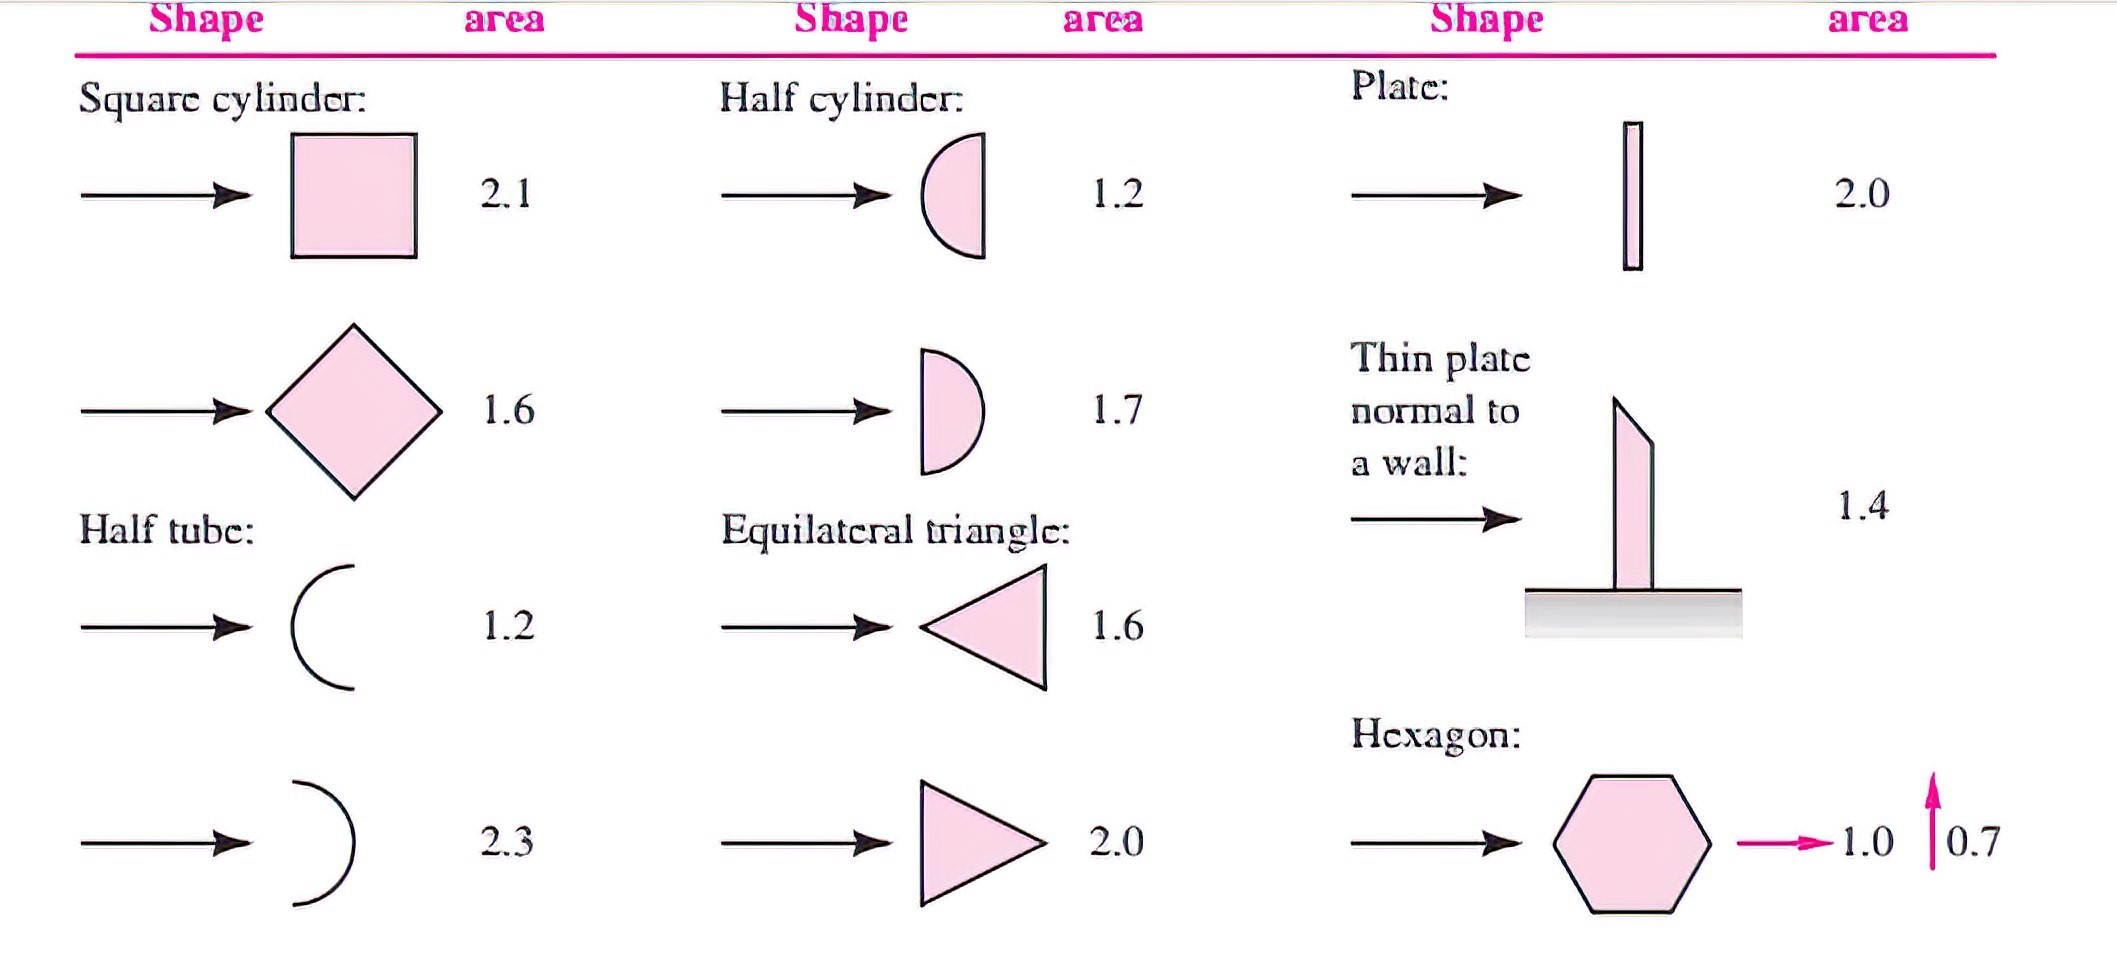
\includegraphics[height=5cm,width=8cm]{pink-polygon.jpg}
		\end{minipage}%
		\begin{minipage}[c]{0.5\textwidth}
			\centering
			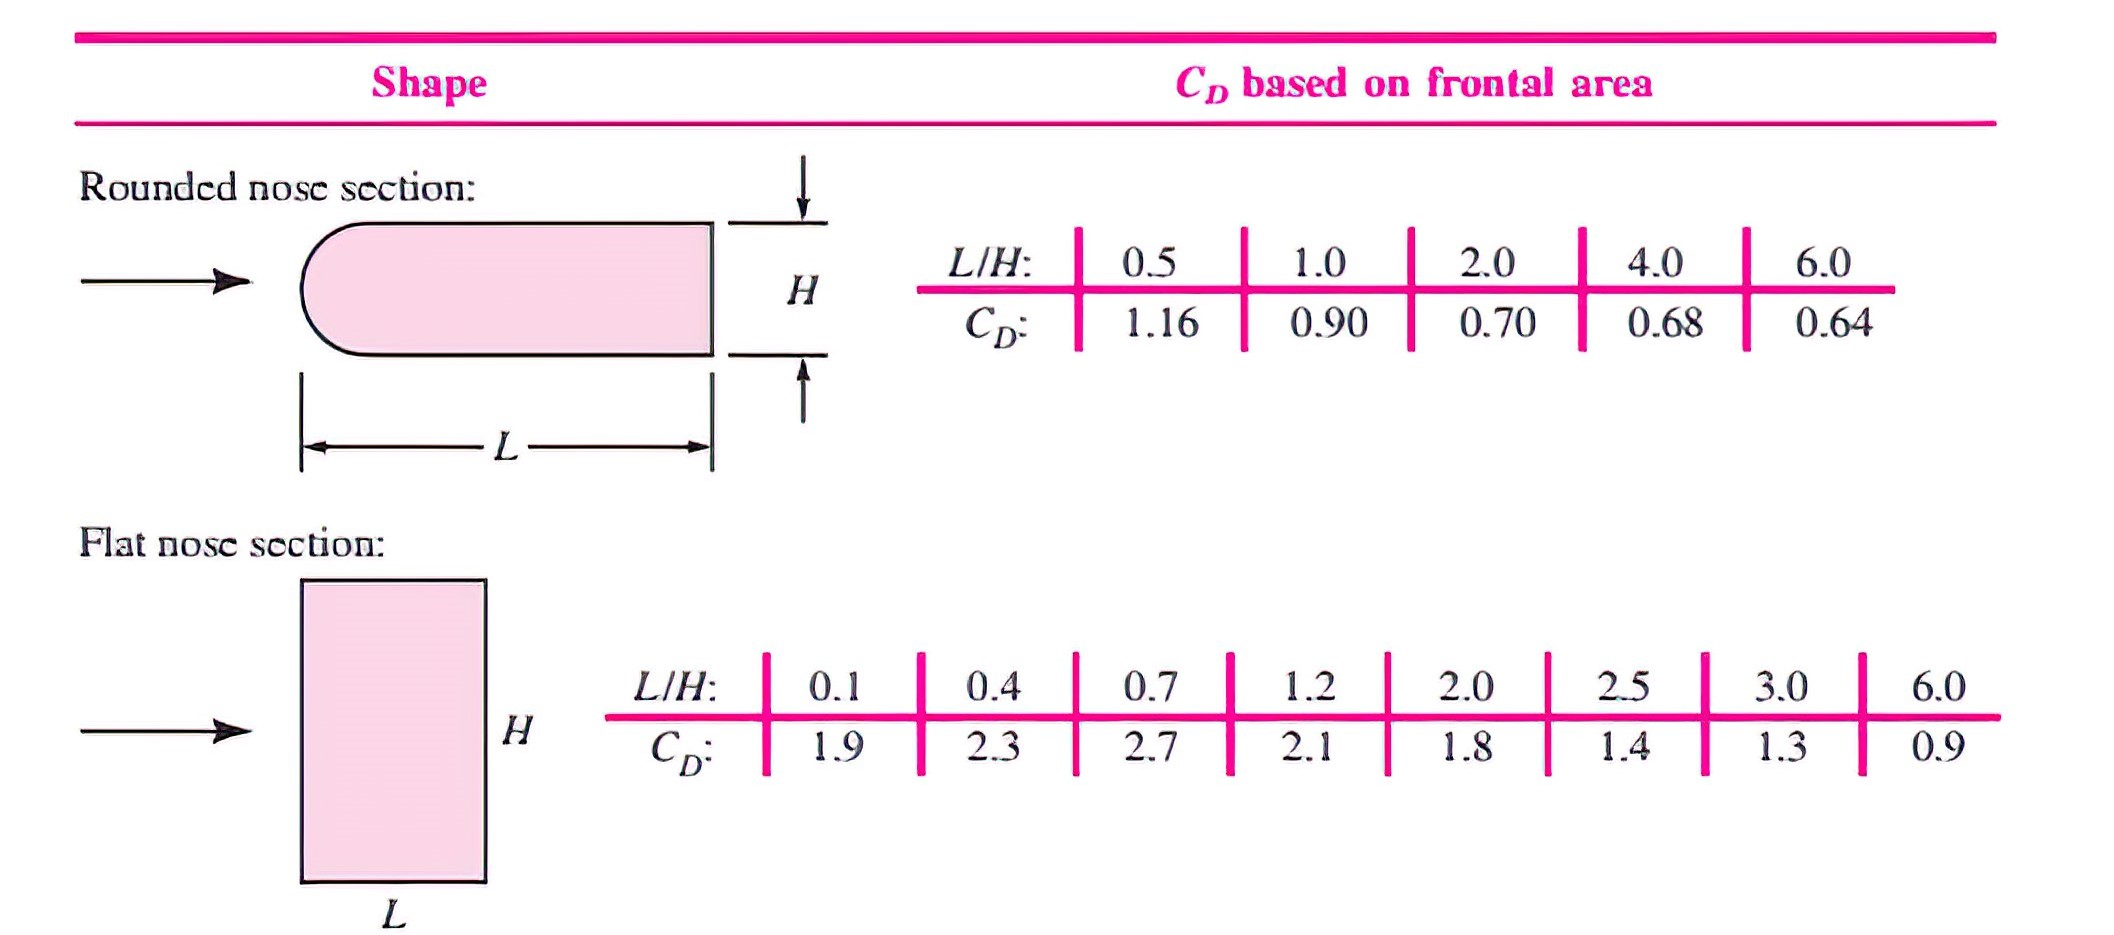
\includegraphics[height=5cm,width=8cm]{pink-section.jpg}
		\end{minipage}
		\centering
		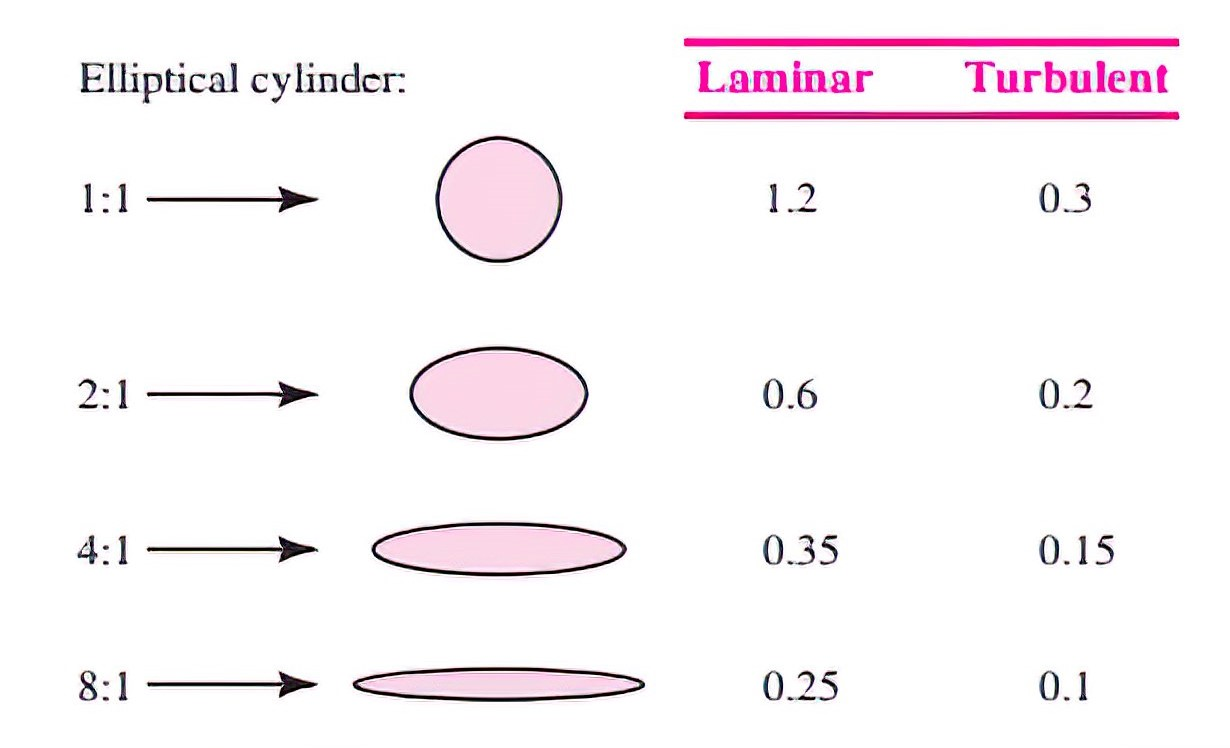
\includegraphics[height=6cm,width=11cm]{pink-oval.jpg}
		\caption{Common Fluid Impact Model}
	\end{figure}
	
	In all the common 2D models in Fig. 1, we can see that the $C_{d}$ of the ellipse model is small, so we can first determine that the horizontal section of our 3D model is an ellipse. Then we chose an elliptical cylinder as the model($H_0$ in height).
	
	Under the premise of using this model, we can guarantee that each horizontal section of the model front view is an ellipse and consider its forces as a whole. The force surface of the model is the surface ACFDBEA(shown in Fig. 2),and its area is as follows(We define $S_{ACFDBEA}$ as the area of surface ACFDBEA, define $C_e$ as the perimeter of ellipse bottom):
	
	\begin{equation}
	S_{ACFDBEA} = \frac{1}{2}  C_e  H_0
	\label{eq_pagerank}
	\end{equation}
	
	\clearpage
	\begin {figure}[htb]
	\centering % 居中显示
	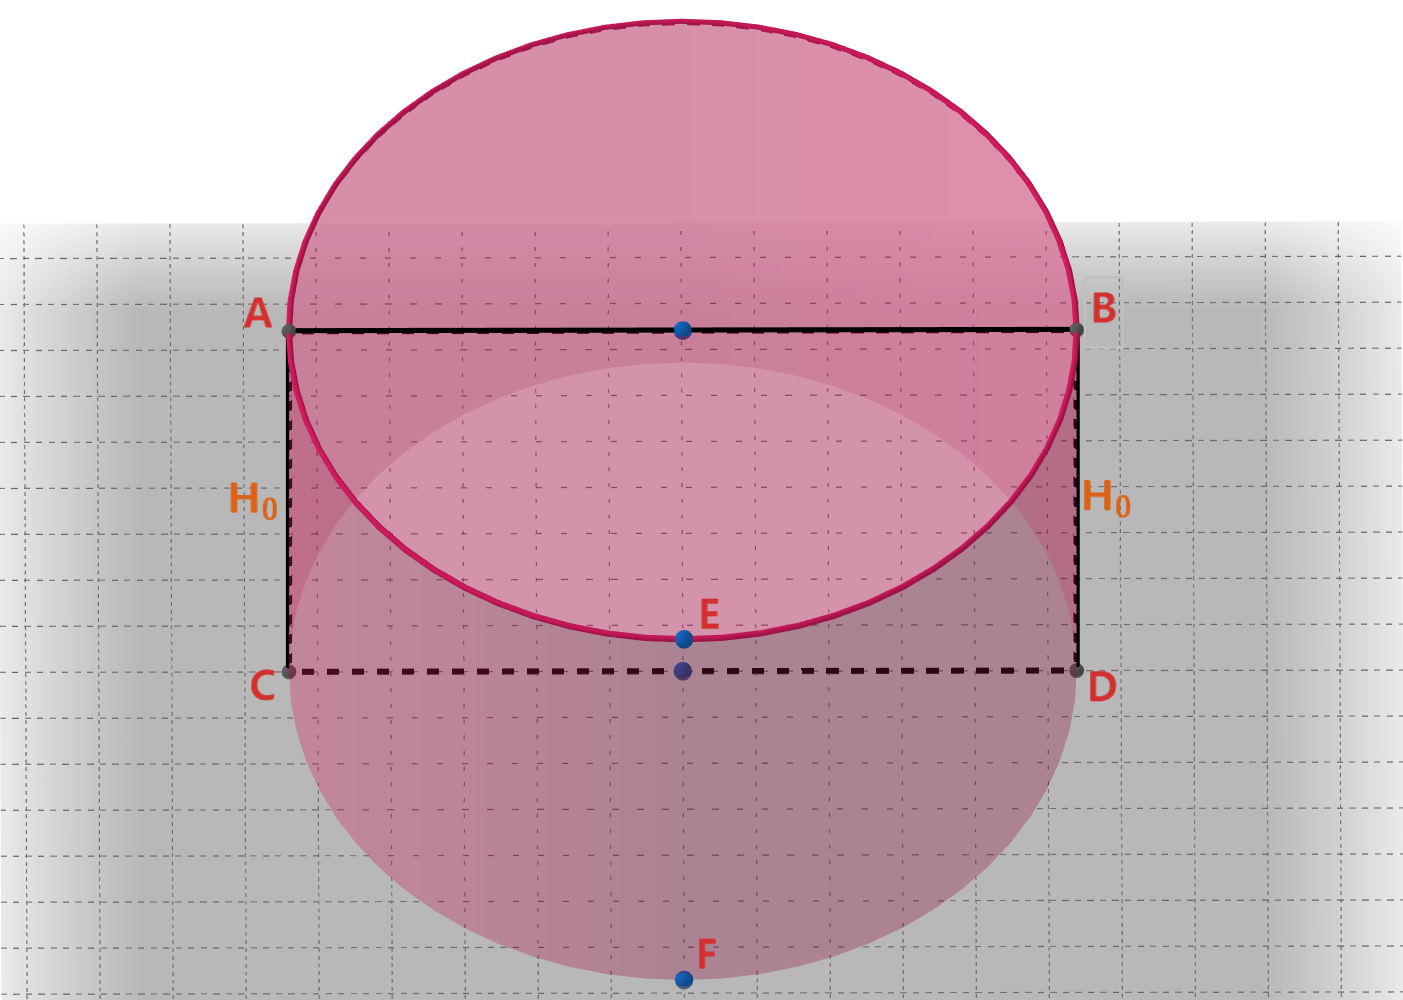
\includegraphics[width=8cm,height=6cm]{Top_v1.png}
	\caption{Top view of  elliptical cylinder} % 标题
	\label{spread_rate}
	\end {figure}
	
	But according to the decomposition rules of force and knowledge of calculus, we can get that the impact force of water will do the same work on surface ACFDBEA and surface ABCD within unit time.
	
	So when F is working on surface ACFDBEA, we can calculate the work done on surface ACFDBEA by calculating  the work done on surface ABCD.
	
	We can easily get the size of ABCD(Here we define $S_{ABCD}$ as the area of surface ABCD, define $L_{Sa}$ as the short axis length at the bottom of the elliptical cylinder):
	
	\begin{equation}
	S_{ABCD} = L_{Sa}  H_0
	\label{eq_pagerank}
	\end{equation}
	
	Therefore, according to Eq. (1), the impact force on the elliptical cylinder model is(We define $F_{model1}$ as the impact force on the elliptical cylinder model):
	
	\begin{equation}
	F_{model1} = \frac{1}{2}  {\rho}  {u^{2}}  C_{d}  L_{Sa}  H_0
	\label{eq_pagerank}
	\end{equation}
	
	%换了一种模型,换成椭圆圆台
	
	Under the premise that the horizontal section of the new model is an ellipse, we chose an elliptical platform with the same height($H_0$) as the previous elliptical cylinder, and made the upper and lower bottom of the model tangent in the top view at the endpoints of the long axis which does not contact the water.
	
	The diagram is as follows:
	
	\begin {figure}[htb]
	\centering % 居中显示
	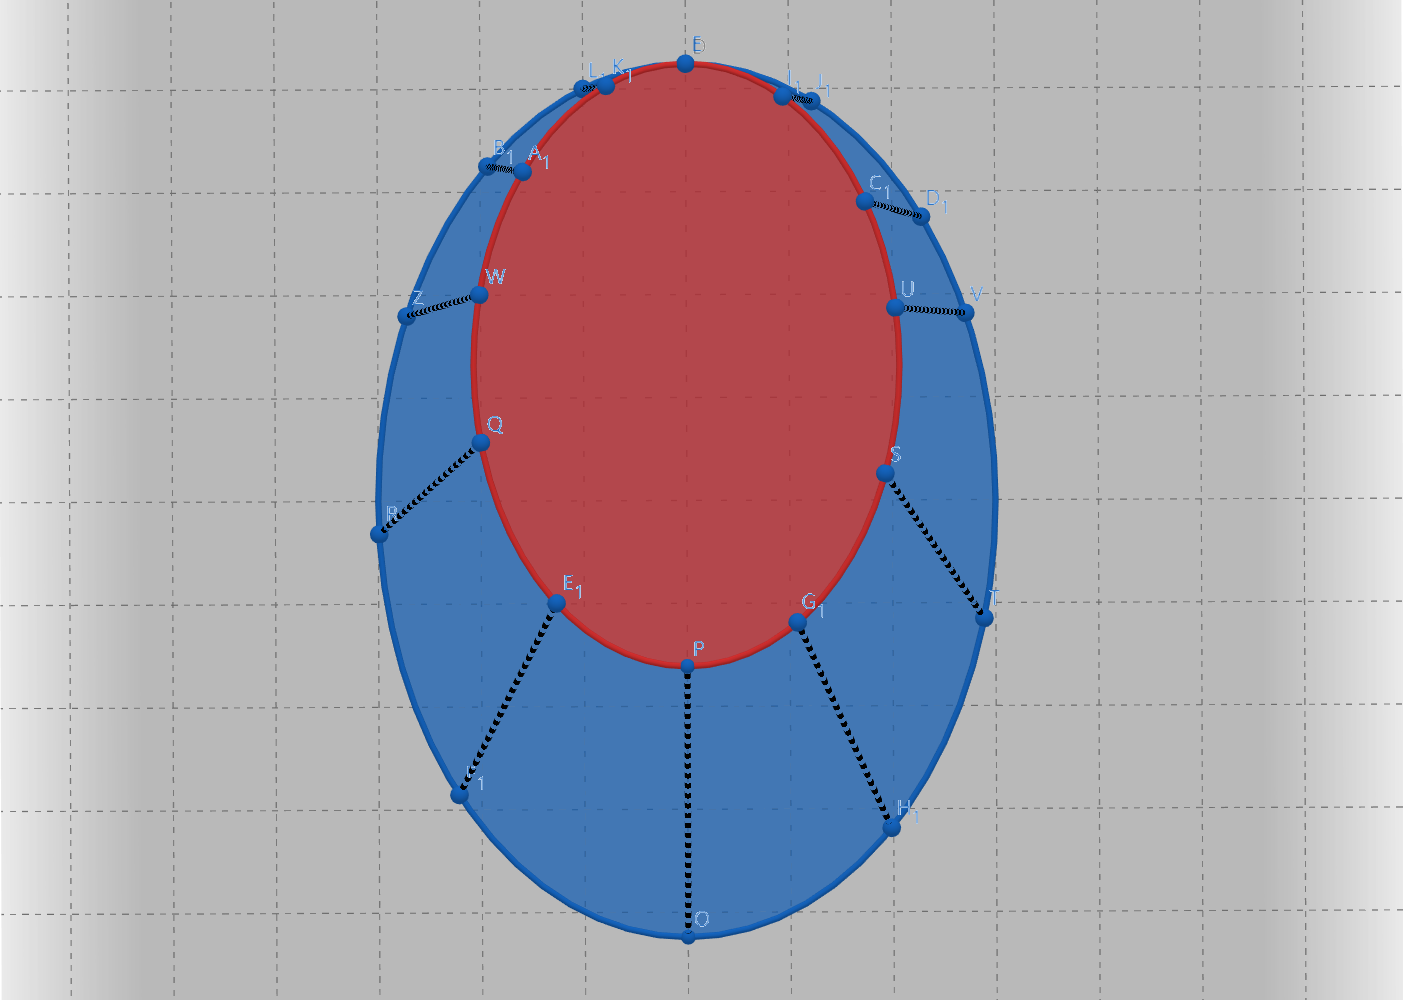
\includegraphics[width=8cm,height=6cm]{Top_v2.png}
	\caption{Top view of elliptical platform} % 标题
	\label{spread_rate}
	\end {figure}
	
	Then, we can also guarantee that each horizontal section of the model front view is an ellipse. But the size of each horizontal section is different, so we analyze a single horizontal section from the perspective of differential.
	
	
	The horizontal section of the model front view is shown in the figure below:
	
	\begin {figure}[htb]
	\centering % 居中显示
	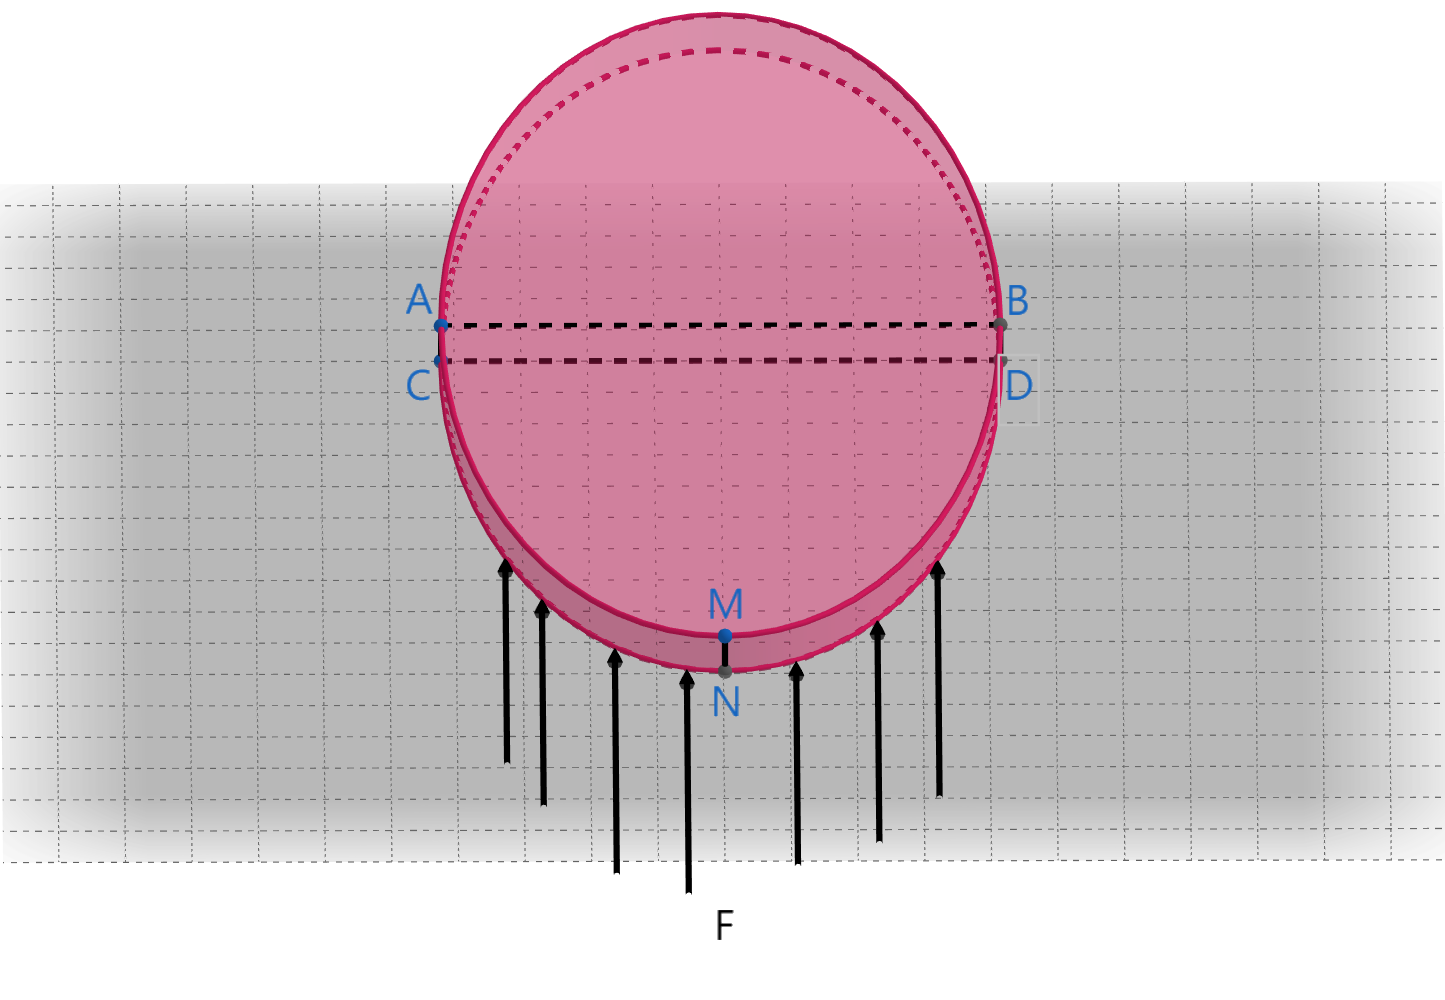
\includegraphics[width=8cm,height=6cm]{overlook_sd.png}
	\caption{overlook section diagram} % 标题
	\label{spread_rate}
	\end {figure}
	
	As shown in Fig. 4, in a cylinder with a height of ${\Delta}h$ formed by pulling up the horizontal section of the model, the force surface is the surface ACNDBMA(Here we define $\Delta$S as the area of surface ACNDBMA, define ${C_e}'$ as perimeter of any ellipse), so the area of surface ACNDBMA can be obtained:
	
	\begin{equation}
	{\Delta}S = \frac{1}{2}  {C_e}'  {\Delta}h
	\label{eq_pagerank}
	\end{equation}
	
	Like we did before, we can replace $\Delta$S equivalent to $\Delta$S'(we define $L_{RT}$ as the minor axis length of the horizontal section ellipse):
	
	\begin{equation}
	{\Delta}S' = L_{RT}  {\Delta}h
	\label{eq_pagerank}
	\end{equation}
	
	In this way, according to Eq. (1), we can quickly get the expression of the force acting on the surface ABCD(We define it as ${\Delta}F$) as below:
	
	\begin{equation}
	{\Delta}F = \frac{1}{2}  {\rho}  {u^{2}} C_{d}  L_{RT}  {\Delta}h
	\label{eq_pagerank}
	\end{equation}
	% 将CD长用h表示
	And in any horizontal section($h$ from the bottom of the model), $L_{RT}$ can be expressed as(We define $L_{Bsa}$ as the short axis length at the bottom of the elliptical platform($AB$ in Fig .5), $L_{Tsa}$ as the short axis length at the top of the elliptical platform($CD$ in Fig .5)):
	
	\begin {figure}[htb]
	\centering % 居中显示
	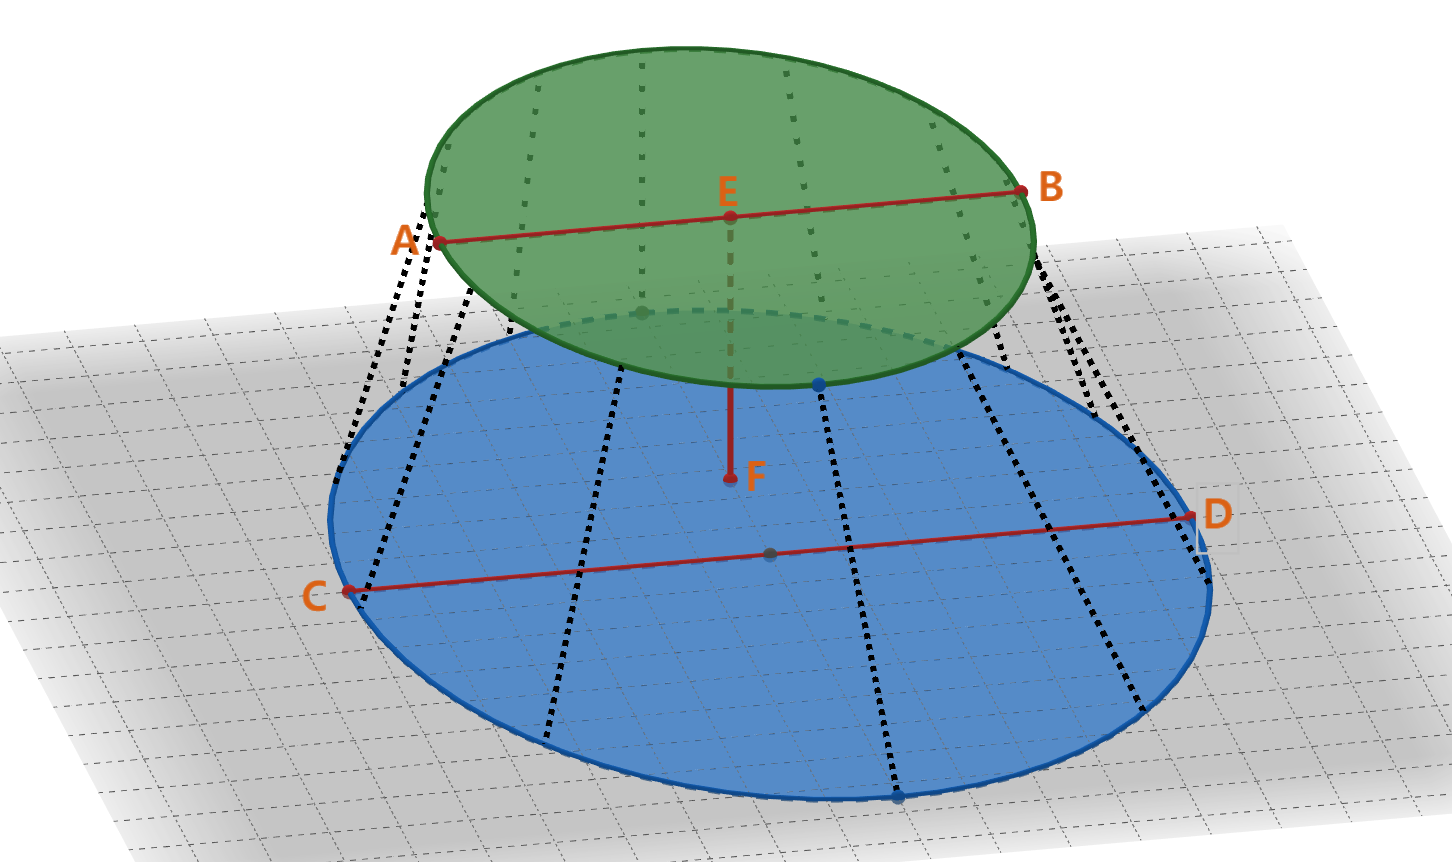
\includegraphics[width=8cm,height=6cm]{Side_v.png}
	\caption{Side view of model} % 标题
	\label{spread_rate}
	\end {figure}
	
	\begin{equation}
	L_{RT} = L_{Tsa} + \frac{H_0 - h}{H_0}  (L_{Bsa} - L_{Tsa})
	\label{eq_pagerank}
	\end{equation}
	
	So from the overall model, the impact force on the elliptical platform can be obtained by integration(We define $F_{model2}$ as the impact force on the elliptical platform):
	
	\begin{eqnarray}
	% \nonumber % Remove numbering (before each equation)
	F_{model2} &=& \int_{0}^{H_0}{\Delta}F \nonumber \\
	&=& \frac{1}{2} \cdot {\rho} \cdot {u^{2}} \cdot C_{d} \cdot \int_{0}^{H_0} L_{RT} \cdot dh \nonumber \\
	&=& \frac{1}{2} \cdot {\rho} \cdot {u^{2}} \cdot C_{d} \cdot \int_{0}^{H_0} [L_{Tsa} + \frac{H_0 - h}{H_0} \cdot (L_{Bsa} - L_{Tsa}) \cdot] dh \nonumber \\
	&=& \frac{1}{4} \cdot {\rho} \cdot {u^{2}} \cdot C_{d} \cdot (L_{Bsa} + L_{Tsa}) \cdot H_0
	\end{eqnarray}
	
	Then by comparing $F_{model1}$ and $F_{model2}$ with Eq. (5) and Eq. (10), it is not difficult to conclude that $F_{model2}$ is smaller than $F_{model1}$, so an elliptical platform model should be used.
	
	\textbf{\subsection{Model Simulation and Analysis}}
	
	As for the specific shape of the ellipse, we can get a set of data from the ellipse related table in Fig. 1 and analyze it.
	
	We used interpolation to analyze this set of data, rendered two sets of function images obtained(shown in Fig .6). So we can learn from the function image(we defined $R_e$ as the ratio of the long axis and the short axis of the Elliptical section of the model): as the $R_e$ increases, the rate of $C_d$ decrease gradually reduces, and approaches 0 when the $R_e$ is 3. Combining feasibility and aesthetics, we can set the $R_e$ to 2.5 - 3.
	
	\clearpage
	\begin{figure}[htb]
		\centering
		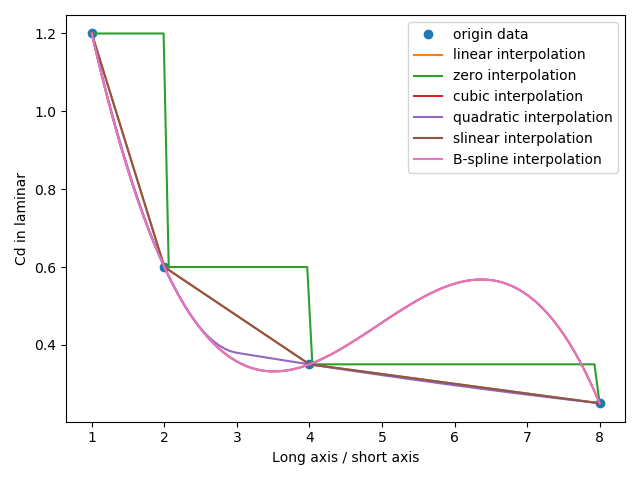
\includegraphics[height=4.5cm,width=10cm]{laminar.png}
		\centering
		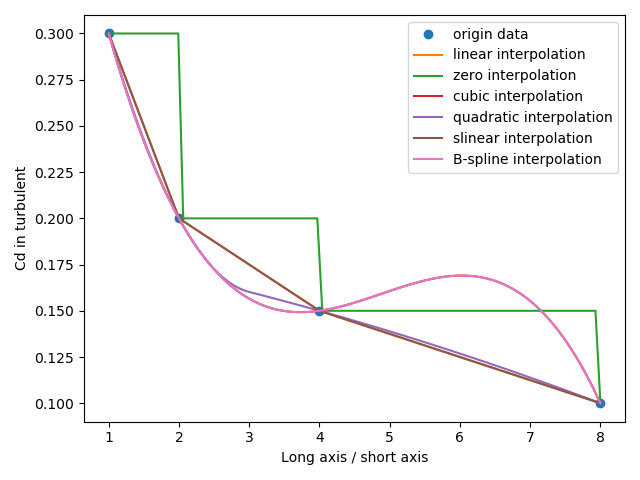
\includegraphics[height=4.5cm,width=10cm]{turbulent.png}
		\caption{Analyze the relationship between the ratio of long and short axes and $C_d$}
		\label{spread_rate}
	\end{figure}
	
	On the other hand, we notice in Fig. 1 that the $C_d$ of half cylinder is lower than Equilateral triangle, and consider the construction problem on the side surface of the model (straight shapes may not be optimal). So we combine the force analysis to conclude that a curved surface on the side may reduce the impact. The force analysis diagram is as follows:
	
	\begin{figure}[htb]
		\centering
		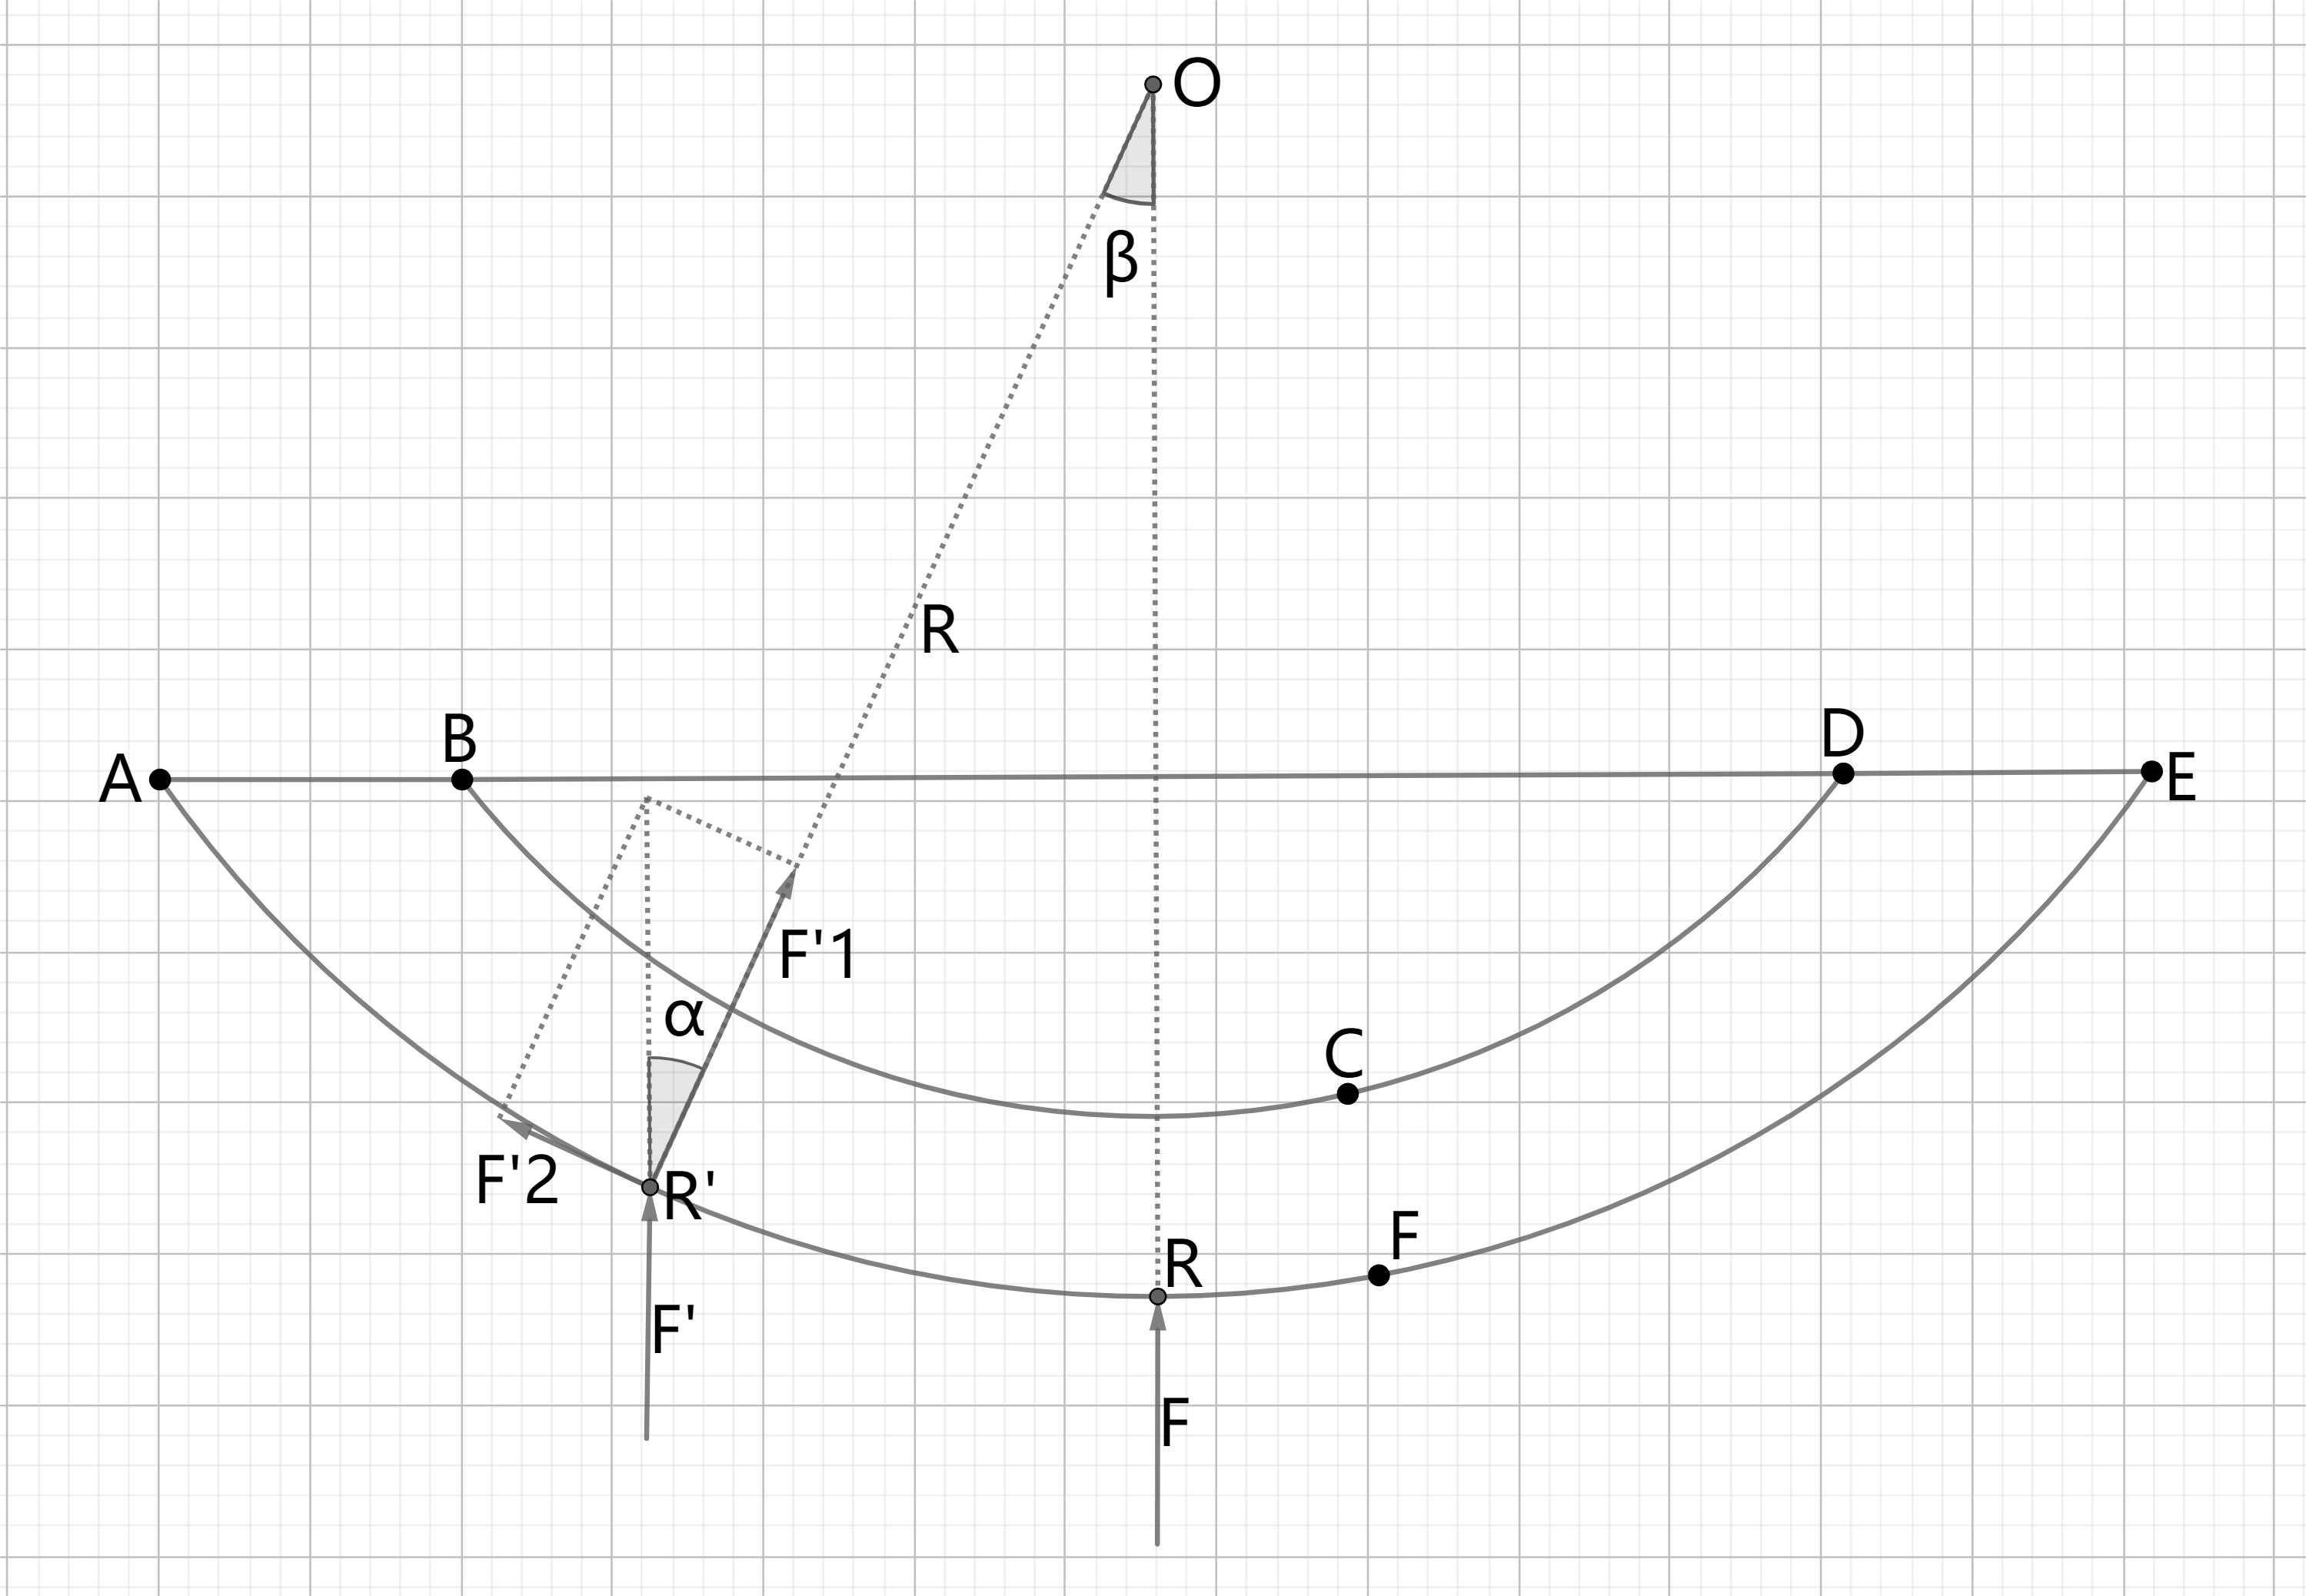
\includegraphics[height=3cm,width=6cm]{Figure2.png}
		\centering
		\begin{minipage}[c]{0.5\textwidth}
			\centering
			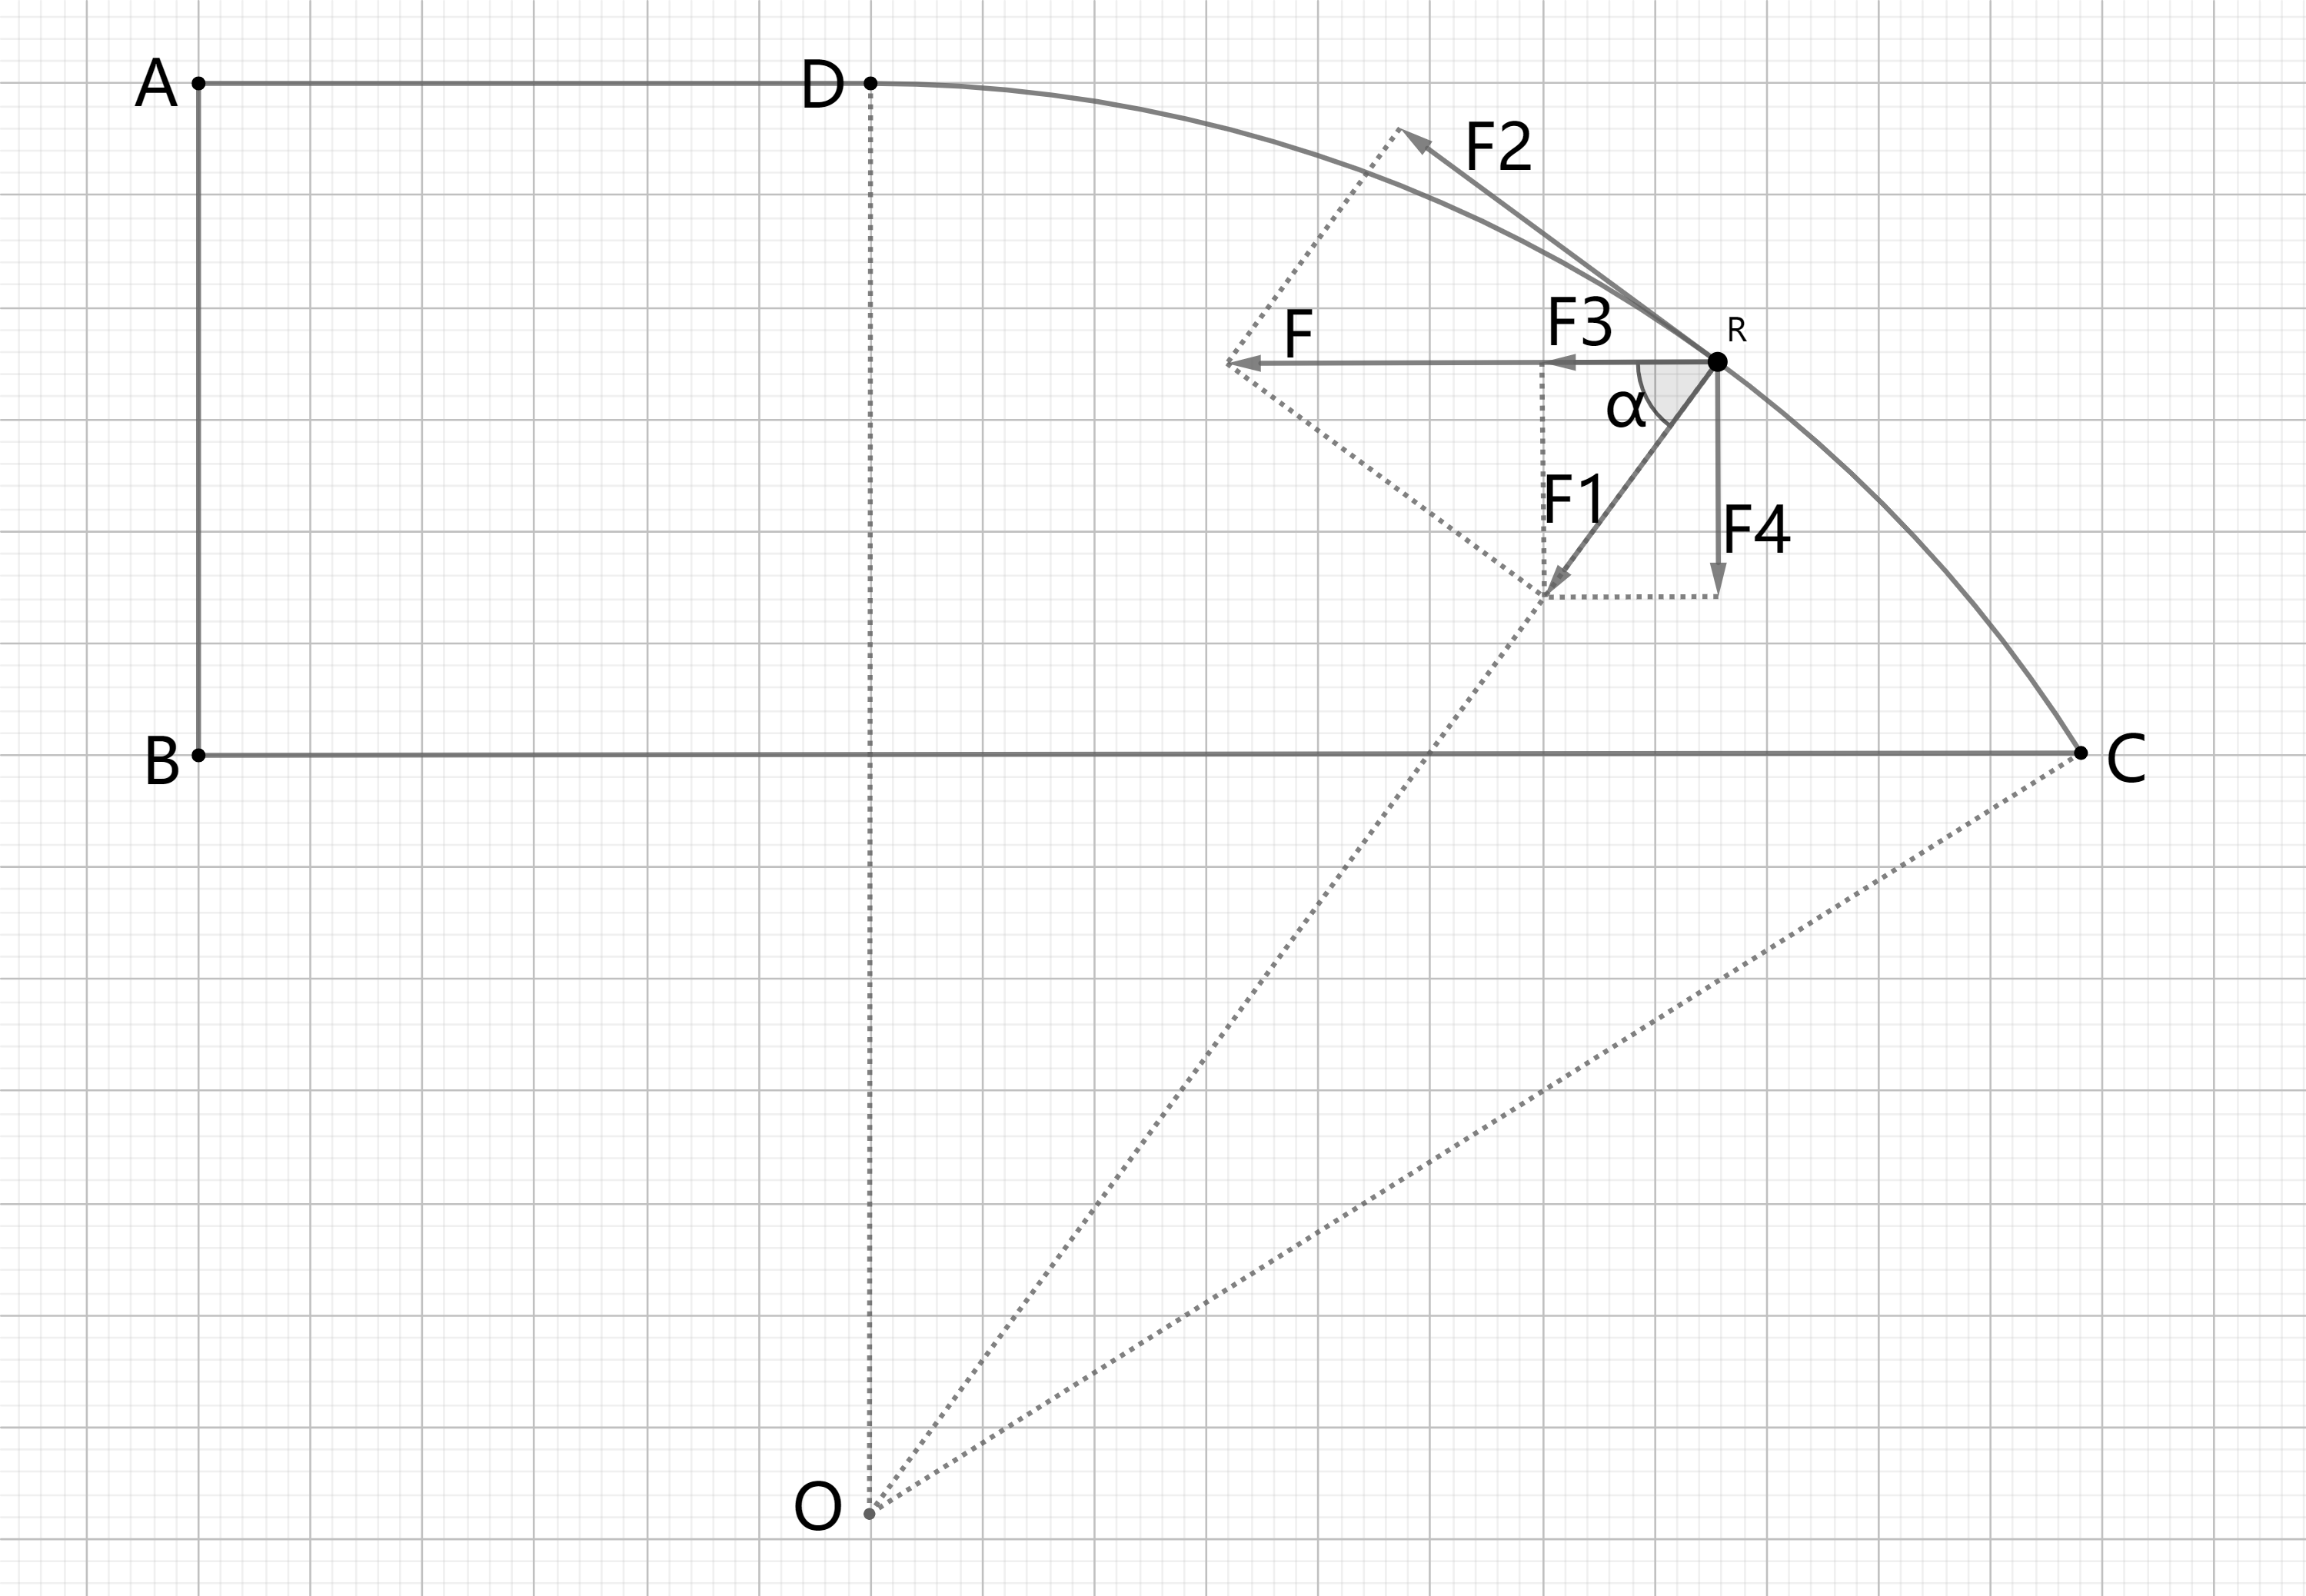
\includegraphics[height=2.85cm,width=5cm]{Figure1.png}
		\end{minipage}%
		\begin{minipage}[c]{0.5\textwidth}
			\centering
			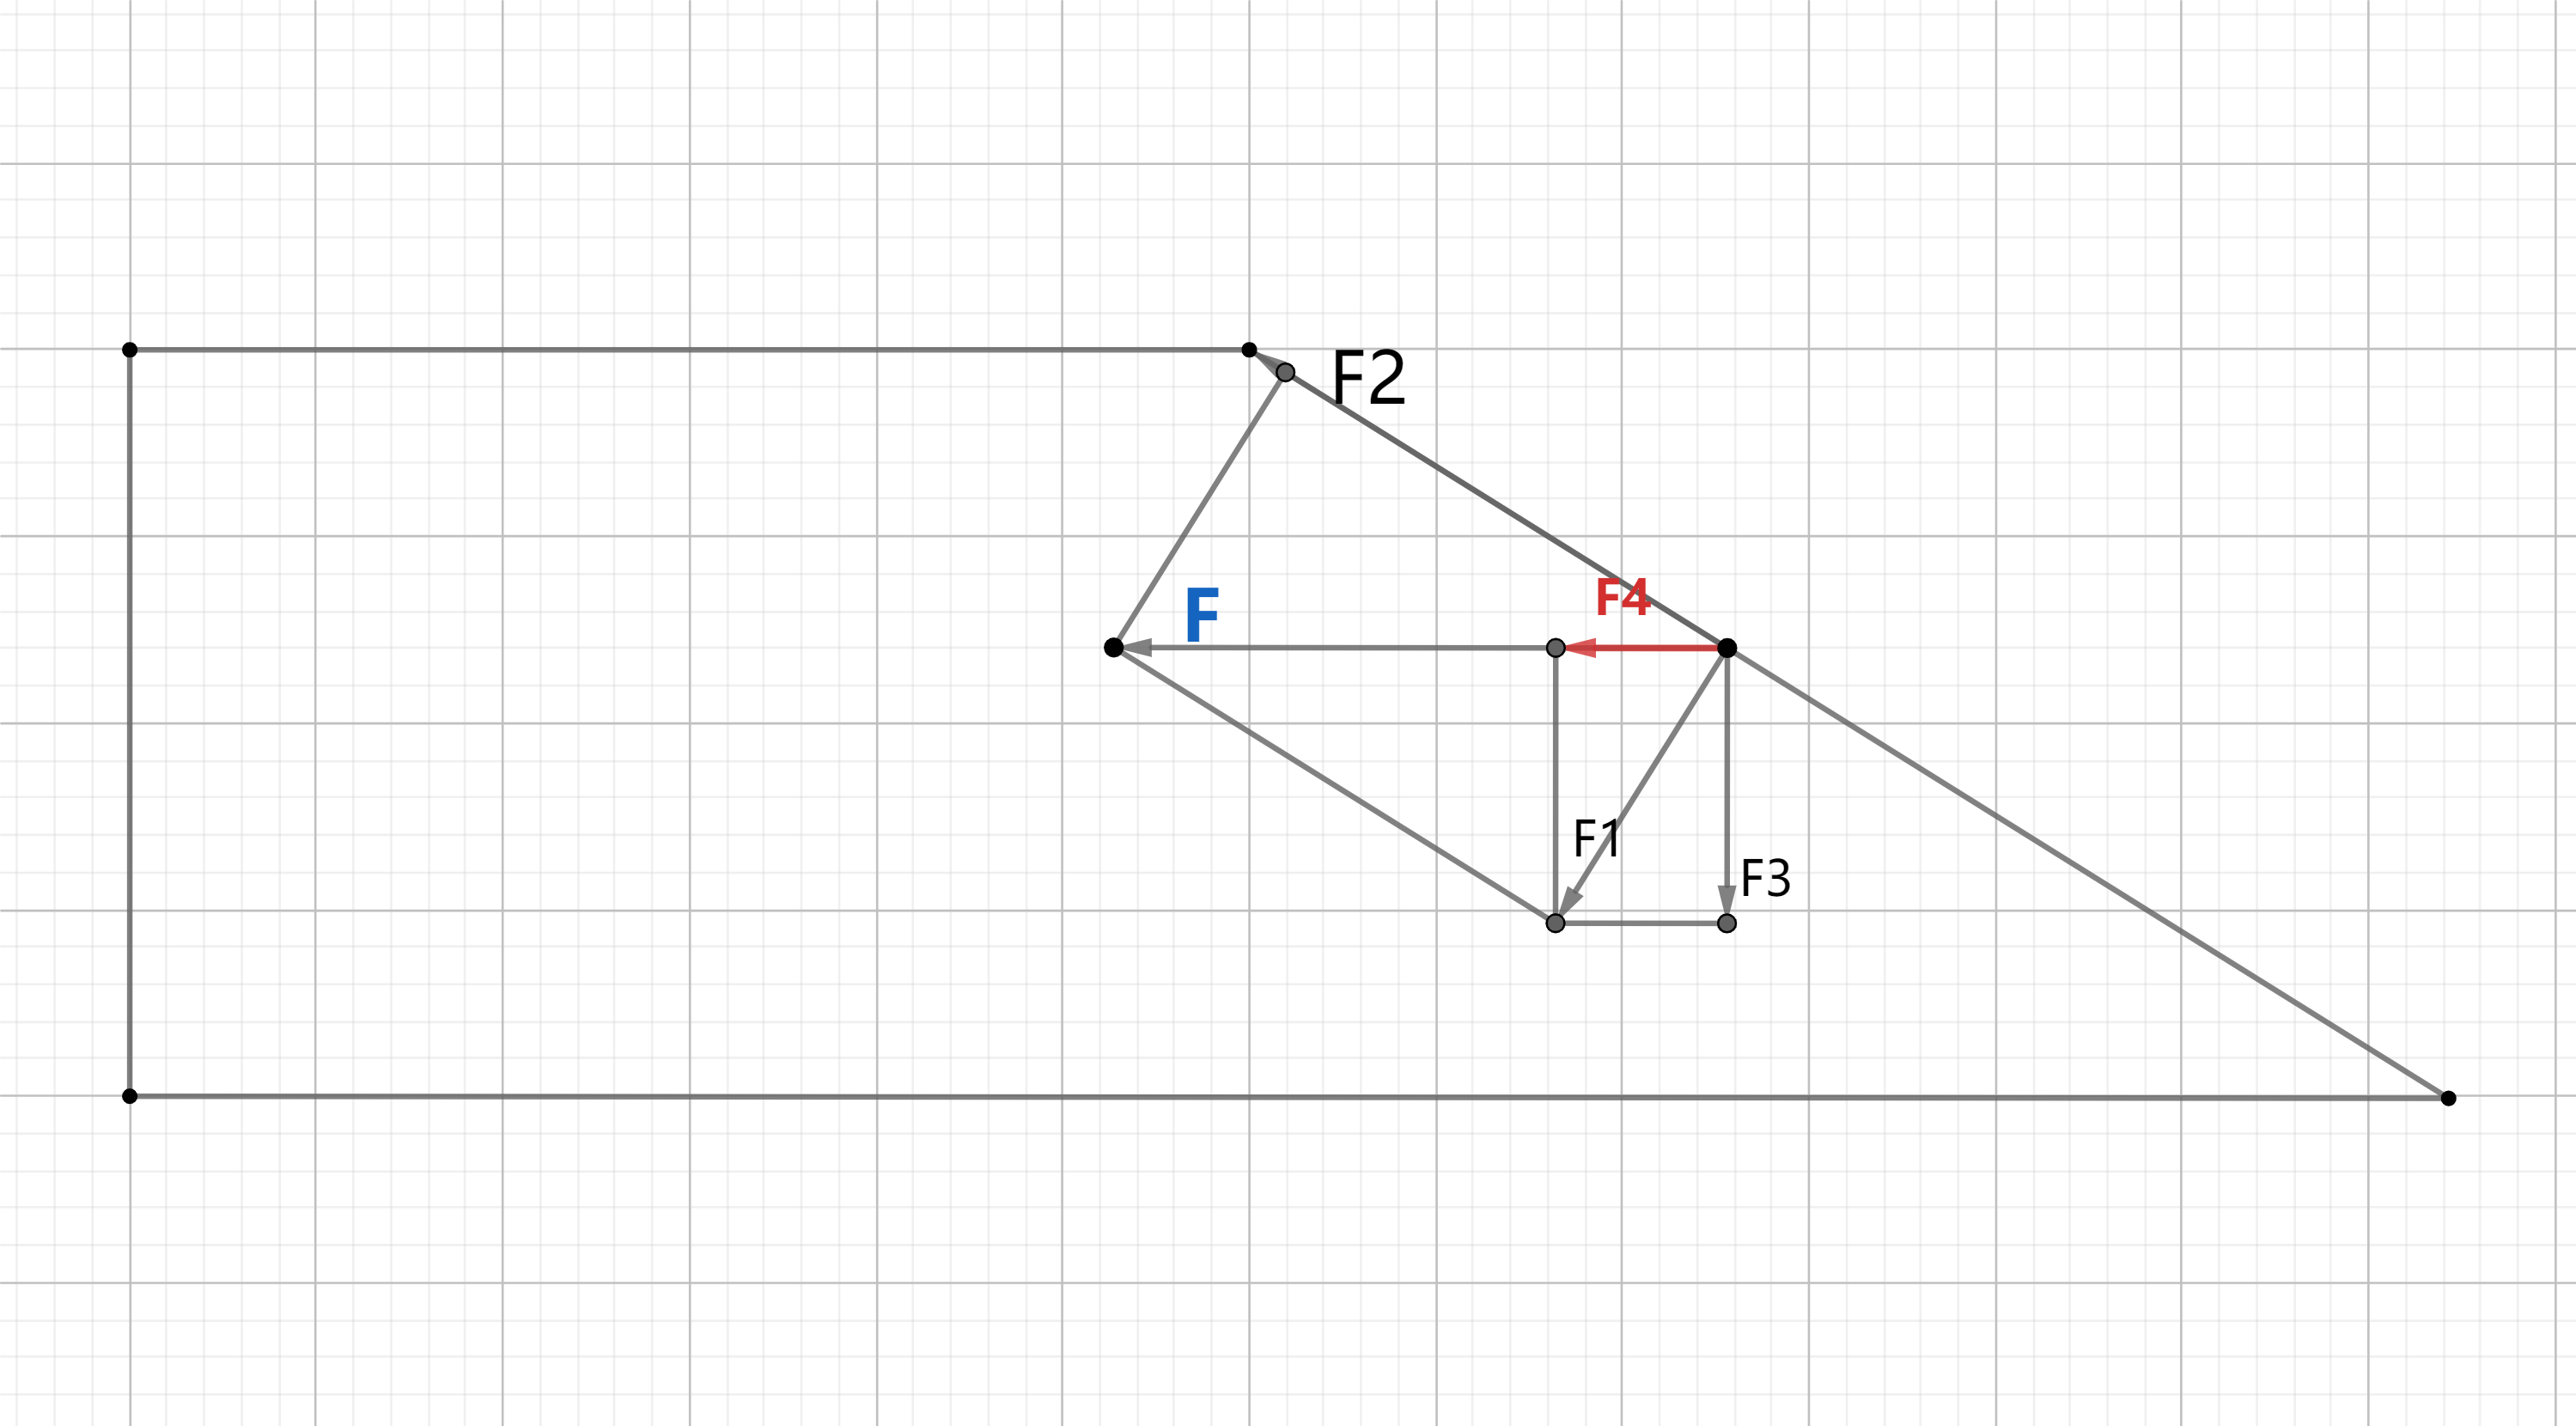
\includegraphics[height=2.85cm,width=5cm]{Figure3.png}
		\end{minipage}
		\caption{Force analysis of vertical section}
	\end{figure}
	
	%吉吉部分
	\textbf{\section{The best proportion of sand and water}}
	%\textbf{\subsection{The liquid bridge model and unit cell structure of wet sand}}
	\textbf{\subsection{Cohesion between two spheres}}
	
	\subsubsection{Meniscus formation}
	Liquid surface tension and capillary action can cause cohesion between wet particles\cite{MitaraiWet}. At the same time, it is considered that  liquid having a pressure of $P_l$ forms a meniscus under the action of air having a pressure of $P_a$. If the radius of curvature between liquid and air is $r_{1}$ and $r_{2}$ ,then the $\Delta P$ can be given by the Young-Laplace equation as
	
	\begin{equation}
	\Delta P = P_{a} - P_{l} = \gamma[\frac{1}{r_{1}}+\frac{1}{r_{2}}]
	\end{equation}
	
	where the $\gamma$ is the surface tension between air and liquid.
	
	\subsubsection{Liquid bridge model between two particles}
	Liquid bridge between two particles (shown in Fig. 8) causes cohesion\cite{MuAnalysis}. In order to clearly describe the force of water between sand particles, we assume that sand particles can be regarded as spherical particles with the same radius and ignore the effect of gravity.
	
	\begin{figure}[htb]
		\centering % 居中显示
		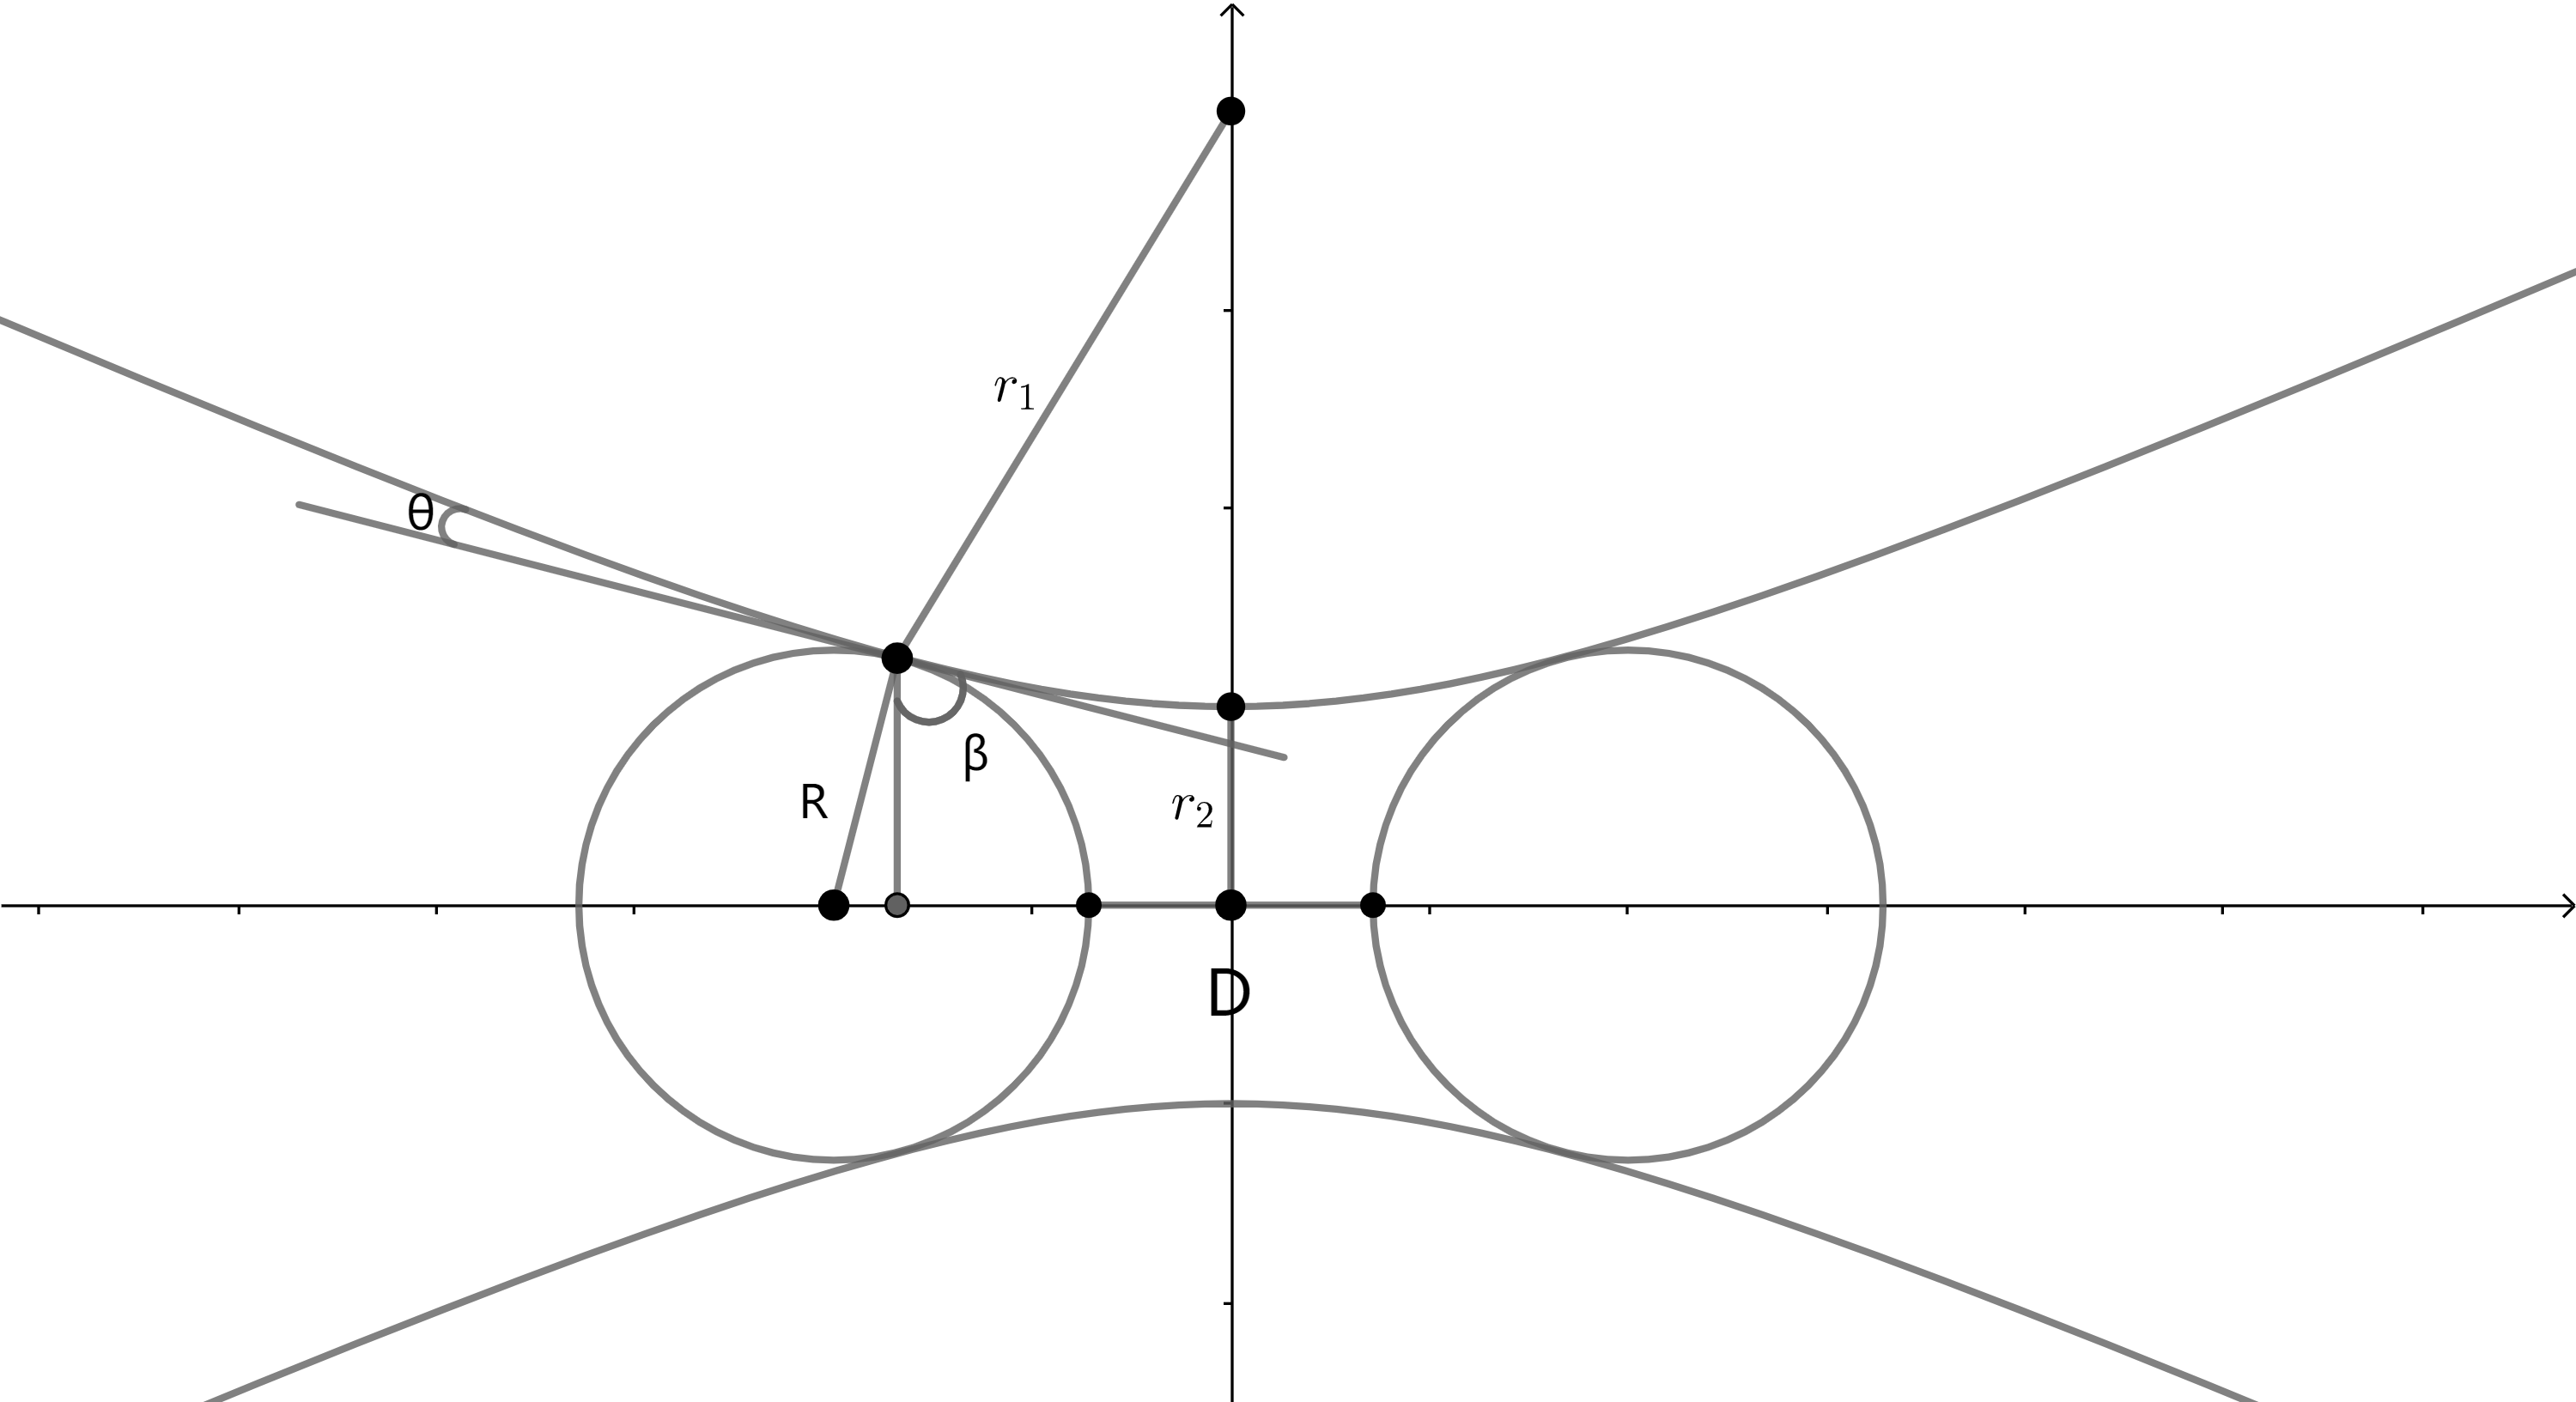
\includegraphics[width=9cm,height=6cm]{bridge.png}
		\caption{Schematic diagram of a liquid bridge between identical spheres} % 标题
	\end{figure}
	
	\subsubsection{Liquid bridge force}
	Because the attractive force between the spheres caused by the liquid meniscus is given by the sum of surface tension and suction\cite{MitaraiWet}, the Dorge method is used to solve the problem of liquid bridge force. The force is given by
	
	\begin{equation}
	F_{bridge} = 2\pi r_{2}\gamma + \pi r^{2}_{2} \Delta P
	\end{equation}
	
	with
	
	\begin{equation}
	\Delta P = \gamma [\frac{1}{r_{1}}-\frac{1}{r_{2}}]
	\end{equation}
	
	From the geometric relationship\cite{MuAnalysis}, we can get
	
	\begin{equation}
	r_{1} = [D/2 + R(1-\cos\beta)]/[\cos(\beta + \theta)]
	\end{equation}
	
	and
	
	\begin{equation}
	r_{2} = Rsin\beta - [1- sin(\beta + \theta)]r_{1}
	\end{equation}
	
	when $ R \gg r_{1} \gg r_{2} $ and $D \ll 2r_{1}cos\theta$, a simplified expression can be written as
	
	\begin{equation}
	F_{bridge} = 2\pi R \gamma \cos\theta [1-\frac{D}{2r_{1}\cos\theta}]
	\end{equation}
	
	Substituting Eq. (14) into Eq. (16),we can get
	
	\begin{equation}
	F_{bridge} = 2\pi R\gamma (\cos\theta - \frac{\cos(\beta + \theta)}{1+\frac{2R(1-\cos\beta)}{D}})
	\end{equation}
	
	Now we qualitatively analyze Eq. (17): On the one hand, we know that $\pi$ and $R$ are constants, and $\gamma$ is a constant under certain conditions. On the other hand, $\theta$ and $\beta$ will change with the change of $D$. When $D$  becomes smaller and the volume of liquid does not change, the contact angle $\theta$ will become smaller, the half-filling angle $\beta$ will become bigger, and the sum of $\theta$ and $\beta$ will become bigger.
	So we can draw the first conclusion that when $D$ becomes smaller and the volume of liquid does not change, $F_{bridge}$ will become bigger. Similarly, the second conclusion is that when the volume of liquid becomes bigger and $D$ does not change, $\beta$ and $\theta$ will have the same change as before and $F_{bridge}$ will get bigger, too.
	We have found similar conclusions in the other literatures and figures to show these conclusions\cite{MuAnalysis}.
	
	Through the following figures(Fig. 9, Fig. 10), we can know the sensitivity of the model: $D $ has a linear effect on $F$; when $ 0 <V <2 \cdot 10^{-8}m ^ 3$ the effect on F is great, and when $V> 2 \cdot 10 ^ {-8}  m ^ 3$ the effect on $F$ is small.
	
	
	\begin{figure}[htb]
		\centering % 居中显示
		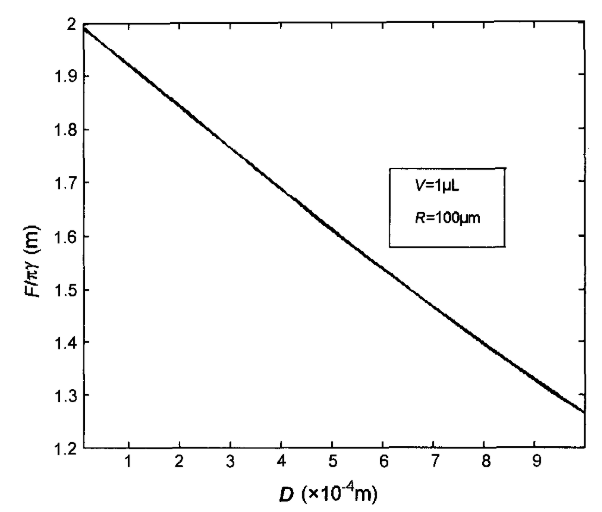
\includegraphics[width=11cm,height=8cm]{bridgeFAD.png}
		\caption{Relationship between liquid bridge force and separation distance}
	\end{figure}
	
	
	\begin{figure}[htb]
		\centering % 居中显示
		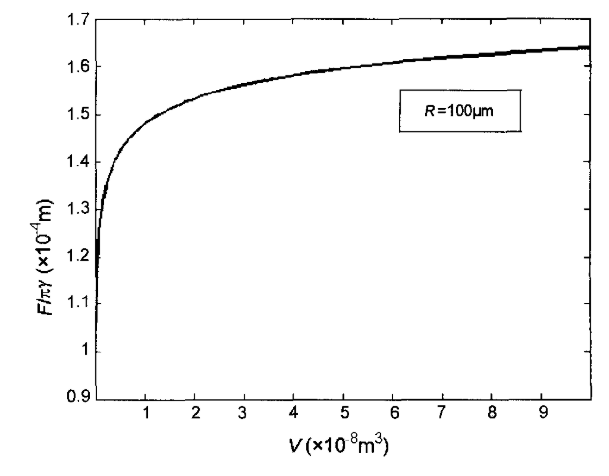
\includegraphics[width=11cm,height=8cm]{bridgeFAV.png}
		\caption{Relationship between liquid bridge force and liquid bridge volume}
	\end{figure}
	
	\subsection{Optimum stress and sand-water ratio}
	Based on these two conclusions, we constructed the following model(shown in Fig. 11) to maximize the cohesion between two particles.
	
	\begin{figure}[htb]
		\centering % 居中显示
		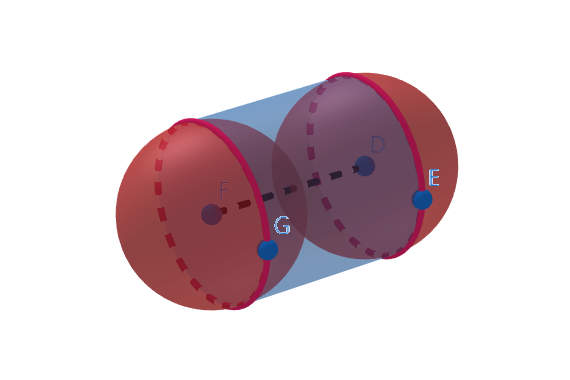
\includegraphics[width=8cm,height=5cm]{maxC.png}
		\caption{Model that can theoretically form maximum cohesion}
	\end{figure}
	
	In this model, the contact angle $\theta = 0$ is for the perfect wet case\cite{MuAnalysis}. When $D\approx 0$, $r_{2} \approx R$, $\Delta P \approx 0$, the liquid bridge force will reach the maximum. It is given that
	
	\begin{equation}
	F_{birdge} = 2 \pi R \gamma
	\end{equation}
	
	and the volume of liquid is
	
	\begin{equation}
	V_{liquid} = \frac{2}{3} \pi R^{3}
	\end{equation}
	
	Then, we extend it to a model in three dimensions. In order to get each particle as close as possible to each other, we refer to the Primitive cubic in the cubic crystal system and built a model of anhydrous sand accumulation(shown in Fig. 12).
	
	\begin{figure}[htb]
		\centering % 居中显示
		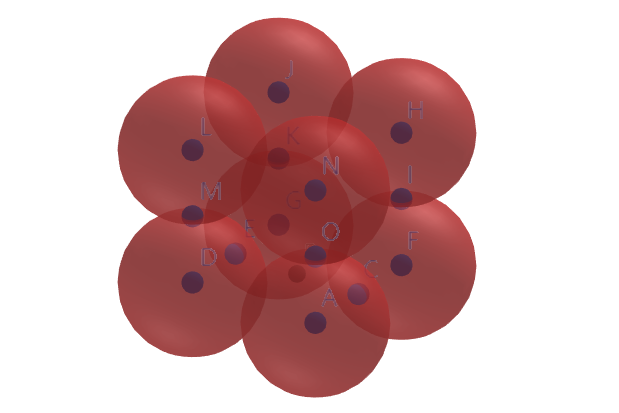
\includegraphics[width=9cm,height=6cm]{Cubic.png}
		\caption{model of anhydrous sand accumulation}
	\end{figure}
	
	Then we add a liquid bridge between two adjacent particles to form the final model in three dimensions(shown in Fig. 13).
	
	\begin{figure}[htb]
		\centering
		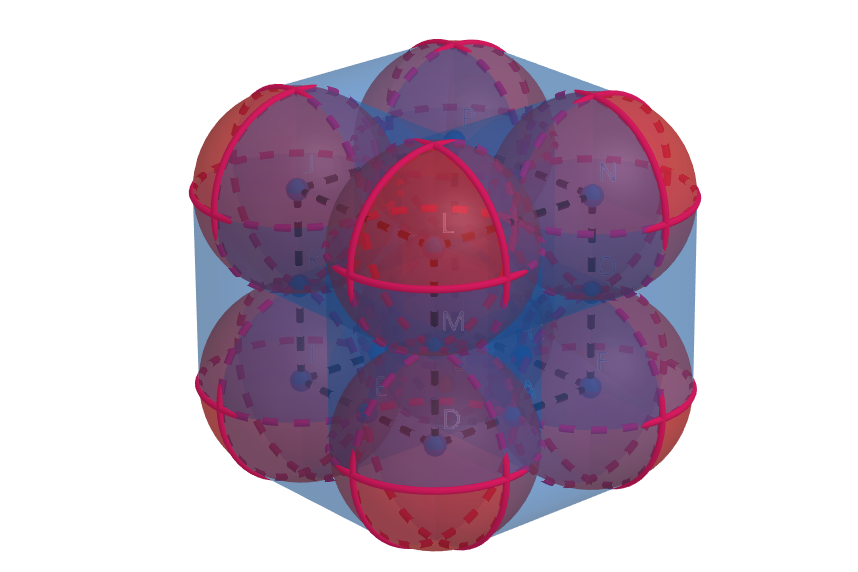
\includegraphics[width=9cm,height=6cm]{fullcubic.png}
		\caption{final model in three dimensions}
	\end{figure}
	
	At this time, the volume ratio of sand to water is given that
	
	\begin{equation}
	\frac{V_{sand}}{V_{water}} = \frac{\frac{4}{3}\pi R^{3}}{8R^{3}-\frac{4}{3}\pi R^{3}}=\frac{\pi}{6-\pi} \approx 1.099
	\end{equation}
	
	The main component of sand is silicon dioxide. So we take the density of sand as 2.65g/cm3. The sea water on the coastline is exposed to direct sunlight so the temperature is high and the salt content is low. According to this reason, we take the density of seawater as 1.02g/cm3. So the mass ratio of sand to water is given that
	
	\begin{equation}
	\frac{m_{sand}}{m_{water}} = \frac{\rho_{sand}V_{sand}}{\rho_{water}V_{water}}=\frac{2.65\pi}{1.02(6-\pi)}  \approx 2.855
	\end{equation}
	
	As a conclusion, the volume ratio of sand to water is about 1.099 and the mass ratio of sand to water is about 2.855.
	
	
	%吉吉部分
	\textbf{\section{Impact of rainwater and model adjustment}}
	
	\textbf{\subsection{Effect of water content}}
	
	In section 4, we have built a model that the water almost fills the gap between sand particles to get greater cohesion. However, under the effect of rain, the content of water will increase directly, which will make the gap between the particles to become larger. In terms of what we've concluded before, if the gap becomes larger, the force of liquid bridge will be smaller which makes the looseness of the sand increase.
	
	Therefore, if the area where the beach is located is rainy, we can consider reducing the water content of the wet sand to get more water absorption under the premise of ensuring the stability of the sand castle.
	
	\textbf{\subsection{Effect of water current}}
	
	When rainwater falls on the slope of the foundation, water flow will be formed. Under certain water flow conditions, the static equilibrium state of the sand will be damaged, and it will change from static to dynamic. So we need to discuss the critical conditions of sand changing from static to dynamic. The movement of water flow on the slope can be decomposed into three directions. We refer to the model of incipient conditions of sediment particle slipping on the slope established by MA Zi-pu et al\cite{马子普Discussion}.
	
	In the model, the speed of the water flow is decomposed into speeds in three directions(shown in Fig. 14).
	
	\begin{figure}[htb]
		\centering
		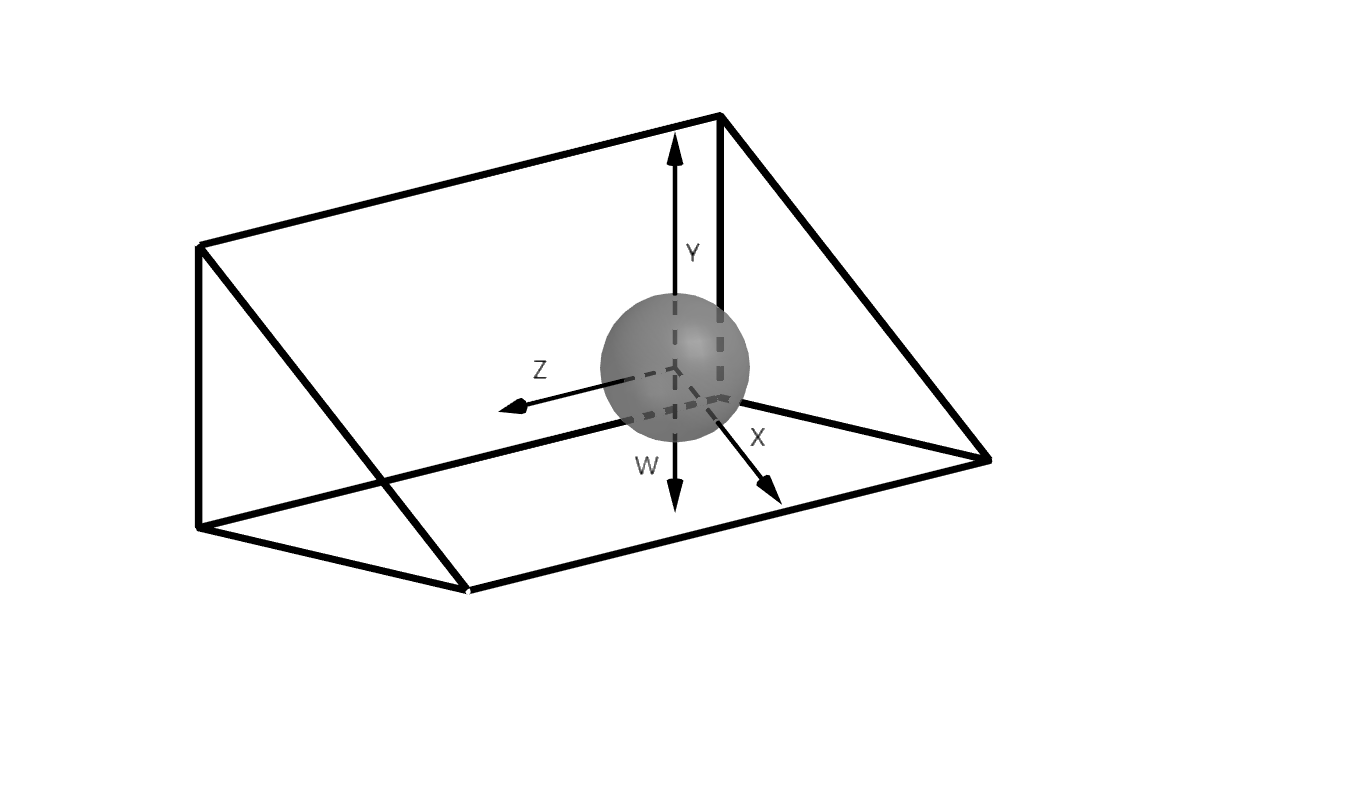
\includegraphics[width=6cm,height=4cm]{20200308002859.png}
		\caption{Sketch of 3D Cartesian coordinate system on slope}
	\end{figure}
	
	According to the right-hand rule, the direction of the parallel slope downward is the positive direction of the X-axis, the direction perpendicular to the slope upward is the positive direction of the Y-axis, and the direction perpendicular to the X-axis and Y-axis and pointing to the reader is the positive direction of the z-axis.
	
	In this paper\cite{马子普Discussion}, the author gives the following three formulas. All these three equations represent the minimum velocity of water that makes sand to slide:
	
	\begin{itemize}
		\item When the main flow is in the x direction
		\begin{equation}
		\centering
		u_{rx} = \sqrt{\frac{2\alpha _{1}d(\gamma _{s}-\gamma)(fcos\theta - sin \theta)}{\rho (\alpha _{3}C_{x}+f\alpha_{2}C_{y})}}
		\end{equation}
		\item When the main flow is in the y direction
		\begin{equation}
		u_{x}^{'} = \sqrt{\frac{2\alpha _{1}d(\gamma _{s}-\gamma)(fcos\theta - sin \theta)}{\alpha _{3}f\rho C_{x}^{'}}}
		\end{equation}
		\item When the main flow is in the z direction
		\begin{equation}
		u_{y}^{'} = \frac{2fW^{'}cos\theta -2\sqrt{W^{2}sin^{2}\theta + {(\frac{\rho d^{2}}{2}\alpha _{3}C_{x}^{'}u_{x}^{'2})}^2}}{f\rho d^{2} \alpha _{2}C_{y}^{'}}
		\end{equation}
	\end{itemize}
	
	the notations involved are the:
	
	$W^{'}$ : effective underwater gravity
	
	$u_{rx}$ : the relative velocity of flow and sediment in the x direction
	
	$u_{x}^{'}$ : the velocity of water ripple in the x direction
	
	$u_{y}^{'}$ : the velocity of water ripple in the y direction
	
	$\gamma_s$ : the volumetric weight of sediment
	
	$\gamma$ : the volumetric weight of water
	
	$C_{x}$ : horizontal drag coefficient
	
	$C_{x}^{'}$ : water ripple's drag coefficient
	
	$C_{y}$ : vertical uplift force coefficient
	
	$C_{y}^{'}$ : water ripple's uplift force coefficient
	
	$\alpha_{1},\alpha_{2},\alpha_{3}$ : Constant, the shape factor of sediment particles(particles are simplified to a sphere, the factor is $\pi/4$ here)
	
	$\rho$ : Constant, the density of water
	
	$d$ : Constant, the grain size of sediment
	
	$f$ : Constant, coefficient(s) of friction
	
	$\theta$  : the angle of slope
	
	\vspace{1cm}
	
	The above three equations indicate the threshold at which the sediment changes from static to dynamic under different flow directions. We can see that if the speed of water is constant, most variables related only to the speed of water are also constant. Then we exclude constants, the only remaining variable in the equation is  $\theta$ , the angle of slope. Through the analysis of the equations, we can know that when $\theta$ becomes smaller, the threshold value will become larger and the difficulty of changing sand particles from static to dynamic will increase. With this conclusion, we can reduce the angle of slope of the model to have a better stability.
	
	%吉吉q3部分结束
	
	%凯凯q3部分
	\textbf{\subsection{Effect of the impacting force of water}}
	
	The impact of rain will take away the sand of the sandcastle model, which is something we cannot ignore.
	
	We can get some data from Papers by Ding Jiaming and Wang Yonghe \cite{丁加明2005雨水冲刷及地表径流对膨胀土路基边坡稳定的影响分析}:
	In the case of heavy rainfall of $50\ mm / h$, we assume that raindrops are water balls with a diameter of $4\ mm$, and have the same speed and mass, and the same time The probability of raindrops falling at every point on the model is the same.
	
	One hour of rainfall in this case, there is $5{\cdot}10^{-2}\ m^3$ rainfall per $m^2$ , which is $1.49{\cdot}10^6$ Raindrops, so the area where raindrops do not coincide with each other is $18.7\ m^2$(we defined it as $S_{Rain}$), each time the rain hits the surface of the model, it will take away the surface sand of $5{\cdot}10^{-4}\ m$(we define ${\L_r}l$ as the thickness of the surface sand removed by a single raindrop).
	
	Falling on the ground of $1\ m^2$ in this case, raindrops will overlap 18 times at the same position; so on the surface of $S_e\ m^2$(we define $S_e$ as the actual area affected by raindrops), raindrops will overlap $S_e{\cdot}S_{Rain}$ times at the same position, in order to simplify the model, we assume that the length of the long and short axes of the ellipse's upper ellipses and the height of the elliptical platform are reduce at a speed of ${\Delta}l$ m/s, so ${\Delta}l$ can be expressed as:
	
	\begin{equation}
	{\Delta}l = L_r {\cdot} \frac{S_e {\cdot} S_{Rain}}{3600}
	\label{eq_pagerank}
	\end{equation}
	
	Because the raindrop force is perpendicular to the ground(shown in Fig .15), it can be easily obtained according to the knowledge of force decomposition and calculus that the surface of the raindrop can be equivalent to the bottom ellipse of the elliptical platform, so $S_e$ can be expressed as(we define $l_{bx}$ and $l_{by}$ as half of the long and short axes of the bottom ellipse of the elliptical platform):
	
	\begin{equation}
	S_e = \pi \cdot l_{bx} \cdot l_{by}
	\label{eq_pagerank}
	\end{equation}
	
%	\clearpage
	
	\begin {figure}[h]
	\centering % 居中显示
	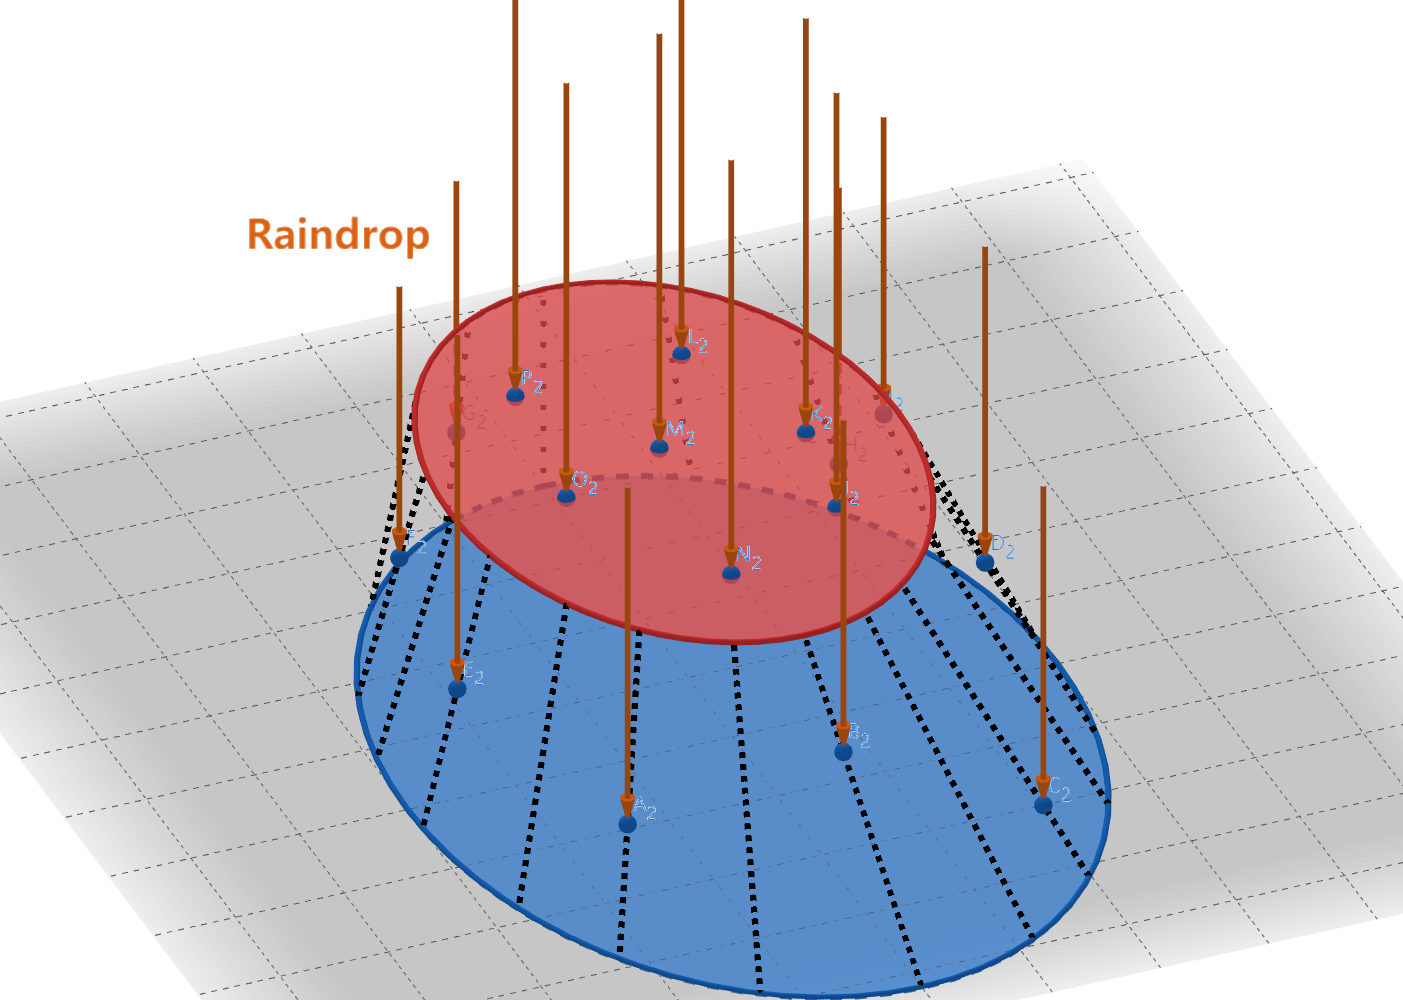
\includegraphics[width=12cm,height=9cm]{raindrop.png}
	\caption{Schematic diagram of rain impact} % 标题
	\label{spread_rate}
	\end {figure}
	
	In this case, ${\Delta}l$ is a constant, from this we can get the expressions of the height of the elliptical mesa and the short axis of the top surface of the ellipse mesa:(we define $H_0$, $H$, $l_{tx0}$, $l_{tx}$ as the origin height of the elliptical platform, the real height of the elliptical platform, half of the origin short axis of the top surface of the ellipse mesa, half of the real short axis of the top surface of the ellipse mesa, and define $t$ as the duration of rain):
	
	\begin{eqnarray}
	% \nonumber % Remove numbering (before each equation)
	H &=& H_0 - {\Delta}l \cdot t\\
	l_{tx} &=& l_{tx0} - {\Delta}l \cdot t
	\end{eqnarray}
	
	We guarantee the ratio of the long and short axes of the top ellipse to 2.5, then we can get the real-time volume of the entire model by integrating(we define $V_{mir}$, ${\Delta}S$, ${\Delta}h$, $h$ as the real-time volume of the model, the area of the horizontal section ellipse and the height of horizontal section ellipse, distance from top):
	
	\begin{eqnarray}
	% \nonumber % Remove numbering (before each equation)
	V_{mir} &=& \int_{0}^{H} {\Delta}S \nonumber \\
	&=& \int_{0}^{H} {\pi \cdot [l_{tx} + \frac{h (l_{bx} - l_{tx})}{H}] \cdot [l_{ty} + \frac{h (l_{by} - l_{ty})}{H}]} \cdot dh \nonumber \\
	&=& \pi \cdot l_{tx} l_{ty} H + \frac{H}{6} \cdot (2 l_{bx} l_{by} + l_{tx} l_{by} + l_{ty} l_{bx} - 4 l_{tx} l_{ty}) \nonumber \\
	&=& 2.5\pi \cdot l_{tx}^2 H + \frac{H}{6} \cdot (5 l_{bx}^2 + 5l_{tx}l_{bx} - 10 l_{tx}^2)
	\end{eqnarray}
	
	In order to test the sensitivity of the model, we set multiple sets of data for $H_0$, $l_{tx0}$ while keeping the model volume constant, and used matplotlib package to draw the function image in python(shown in Fig .16):
	
	\begin {figure}[h]
	\centering % 居中显示
	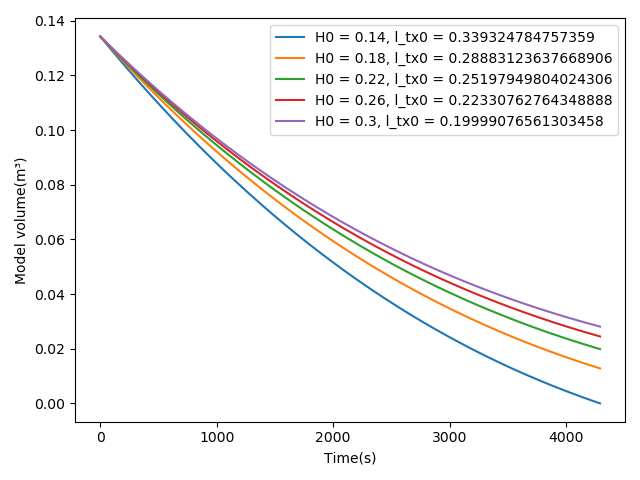
\includegraphics[width=12cm,height=9cm]{rain.png}
	\caption{The process of a sand castle being hit by rain} % 标题
	\label{spread_rate}
	\end {figure}
	
	From the function image, we can see that with the decrease of $H_0$, the rate of model volume decrease becomes larger. The model with $H_0 = 0.14\ m$ has been washed away by rain when the time reaches about 4290 seconds. So while keeping the volume and the area of the bottom ellipse constant, the higher the model is, the more resistant it is to the impact of rain.
	
	%q4部分
	\textbf{\section{The other methods to prolong sandcastles life}}
	
	\textbf{\subsection{Compaction}}
	
	The first way to increase the strength of a sandcastle is to hold the foundation firmly together, to reduce the gaps between the sand in it, to strengthen the intermolecular forces between the sand grains, and to integrate the foundation. An easier way is to fill the sand with a small bucket and press it down with a shovel or fist.
	
	\textbf{\subsection{Build a wall and dig a moat}}
	
	Adding a wall can protect the castle. This can not only reduce the impact of the sea on the sand castle to a certain extent, but also can increase the beauty of the sand castle more solemn
	
	Digging a moat next to the wall. This ditch will retain most of the water when the waves arrive. And the slightly dry sand at the bottom of the ditch can absorb a lot of water.
	
	\textbf{\subsection{Curing agent}}
	
	We can also regard sandcastle as a building. In modern architecture, it is not enough to only use natural materials in nature, and most of them are mixed with additives. If there is a curing agent, the sand castle foundation can be the hardness
	
	\textbf{\section{An Article to Fun in the sun}}
	%(See next two pages)
	%
	%\newpage
	%\thispagestyle{empty}
	%\newgeometry{left = 3.5cm, right = 3.5cm}
	%\centering
	\vspace{2cm}
	%% 设置两端对齐
	\justifying
	\noindent {\centering \fontsize{18pt}{18pt}\selectfont \textbf{How to build a stable sandcastle scientifically}\par}
	
	\vspace{1cm}
	\noindent FROM: Team {} 2013484 , MCM B
	
	\noindent To: Fun in the Sun
	
	\noindent Date: March 08, 2020
	
	\vspace{10pt}
	\fontsize{13}{12.5}\selectfont
	No one could say no to playing sand on the beach. Is there any more interesting than creating a sandcastle step by step? A great day with sandcastle is never be dull.
	
	But every time when your castle be crumbled by waves and tides,have you thought about how to strengthen your castle?
	
	Today I will tell you the secrets of building a perfect long-lived castle using scientific methods!
	
	\textbf{1. The optimum sand water ratio}
	
	The first and most important thing you need to know about sandcastle is that its material is a mixture of sand and water.Only wet sand can be used to build a stable castle.
	
	The principle of this is also well to explained by science.Inside the sand,there are hundreds of millions of sand particles.Water is connected between the sand particles as "bridge".The connection,which we called "Liquid Bridge" ensures structural stability.
	
	When the force between the sand particles reaches the maximum, the sand pile is the closest. In our model calculation, the overall ratio of water and sand is about 1:1.1
	
	\textbf{2. The shape of base}
	
	Playing sand is much more fun than pile a modular Lego.Let sand flow through your fingers and use your imagination to build your castle freely without being bound by the frame.
	
	Whether it's a skyscraper or a sandcastle,needs a sturdy base or bottom.If the bottom isn't strong enough to hold it up,it could crumble or tip over!
	
	You must be thinking about what shape of foundation is the strongest and  the most resistant to the impact of seawater.Is it rectangle?Is it circle?Is it hexagon?
	%\newpage
	%\thispagestyle{empty}
	According to our physical model ,the conclusion is that the best impact-resistant shape is oval.
	
	No matter which part of the ellipse the sea's impact hits,the oval will spread outward with the impact point as the center to ensure every part is under the same pressure,it will not be crushed by the sudden impact of waves.
	
	\textbf{3. Other skills}
	
	In rainy weather, the amount of water added to the sand can be appropriately reduced because the humidity of the air is high. Similarly, in the clear sun, don't forget to sprinkle some water on the outside of the sand castle, otherwise the outer wall of the sand castle will crack, and the future of this powerful city is collapse.
	
	There are other clever ways to ensure the longevity of the sand castle.The construction of city walls and moats can effectively reduce the impact of seawater, and sand castles will look more majestic and tall.
	
	How interesting it is to create a beach castle!When you know these sand casting skills, you will appreciate the charm of science in your next play.
	
	How about go to the beach next time?
	
	\begin{figure}
		\centering
		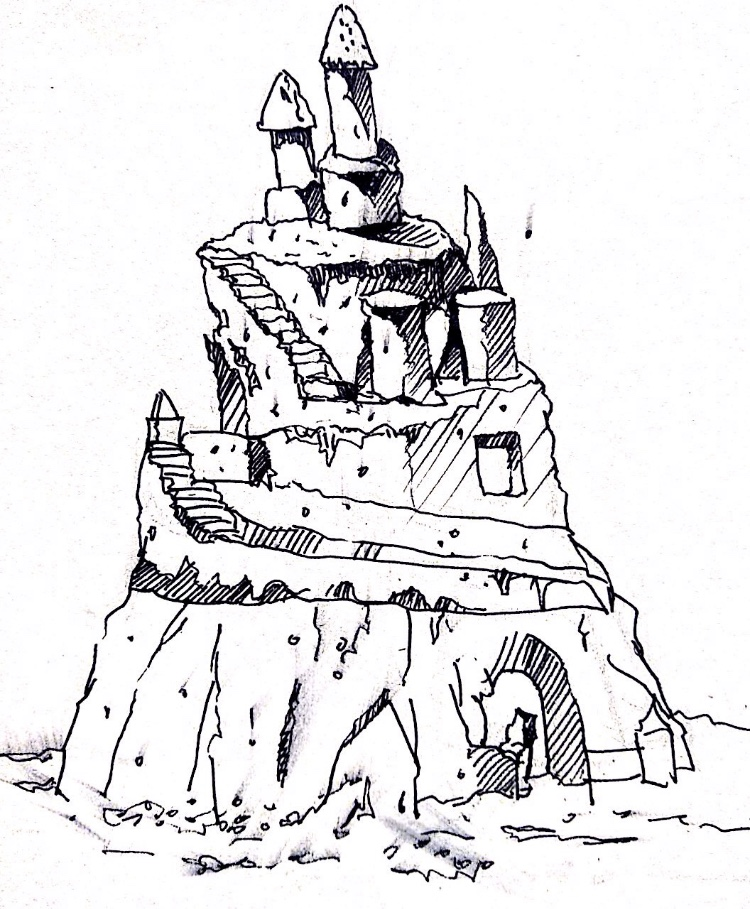
\includegraphics[width=4.875cm,height=6.75cm]{sc.png}
	\end{figure}
	
	
	\newpage
	\textbf{\section*{References}\addcontentsline{toc}{section}{References}}
	\fancyhf{}
	\fancyhead[R]{Page \thepage\ of 28}
	\fancyhead[L]{Team \# 2013484}
	\bibliography{books}
	\Large
	\bibliographystyle{IEEEtran}
	
	\newpage
	\textbf{\section*{Appendices}\addcontentsline{toc}{section}{Appendices for Code and Data}}
	\fontsize{13pt}{12.5pt}\selectfont
	Here is Code we used in our model, which python is the main development language.
	\vspace{7pt}
	\textbf{\subsection*{Appendices A Relationship between the ratio of long and short axes and Cd}}
	\noindent{\rule{\textwidth}{0.2mm}}
	\vspace{-18pt}
	\fontsize{13pt}{12.5pt}\selectfont
	{
		\lstinputlisting[language=python]{Cd_fit.py}
	}
	\vspace{-15pt}
	\noindent{\rule{\textwidth}{0.2mm}}
	\textbf{\subsection*{Appendices B The process of a sand castle being hit by rain(sensitivity analysis)}}
	\noindent{\rule{\textwidth}{0.2mm}}
	\vspace{-18pt}
	\fontsize{13pt}{12.5pt}\selectfont
	{
		\lstinputlisting[language=python]{rain.py}
	}
	\vspace{-15pt}
	\noindent{\rule{\textwidth}{0.2mm}}
	
\end{document} 